\begin{refsection}

\chapter{Development of a Ch-bonding DNA binder}\label{ch:dna-binder}

\section{Introduction}

\subsection{Cancer and treatment}
In Australia, cancer consistently ranks as one of the leading causes of death among all age groups. In 2015, lung cancer alone accounted for 8,466 deaths, which ranked only behind ischaemic heart disease (19,777), dementia (12,625), and cerebrovascular diseases (10,869).
If other cancers are included, the total number of deaths attributable to cancer is 1.5 times those caused by heart disease\autocite{abs2015}.

It has clear and serious consequences among families and communities, and also a wider economic price, costing Australia \$2 billion each year, of which the majority is spent on treatment\autocite{Mathers1998}.
Developing treatments for cancer has therefore attracted significant interest from the pharmaceutical industry, government, and the general public\autocite{Rankin2015}.

Cancer is not a single disease, but an umbrella term which encompasses many different types of malignancies.
The uniting theme among them is the uncontrolled and damaging division of cells.
Because of the diversity of diseases broadly termed ``cancer'', treatments are often difficult to develop and highly specific to one particular class\autocite{Hanahan2011}.

Some more general treatments for cancer exist.
These include surgery and radiation therapy.
While these treatments do have limitations (e.g.\ surgery is only viable for solid tumours), they are usually very effective, and are often combined with more specific therapies where appropriate.


\subsection{Radiation therapy}
Radiation therapy is one such general treatment for cancer.
A course of radiation therapy consists of a series of exposures to radiation (x-rays, generated electrically; $\gamma$-rays, generated by radioactive decay; or, less commonly, fermionic particles such as protons, neutrons or electrons), with the intention of damaging the DNA of the cancer cells beyond the cells' ability to repair, resulting in death of the cells and remission of the cancer\autocite{Ward1994}.
The mechanism of this damage is either direct, where a photon ejects an electron from the DNA polymer itself (via Compton scattering); or indirect, where other molecules (usually water) are ionised by the radiation, generating reactive oxygen species (ROS) such as \ce{^{$\cdot$}OH} and \ce{O_{2}^{-}}\autocite{Ward1988}.

If generated in the vicinity of the nucleus, these ROS may diffuse short distances and abstract electrons from DNA, causing damage to the DNA\autocite{Evans2004}.
Due to the minuscule volume occupied by DNA within the cell, indirect damage is the dominant mechanism in external beam radiotherapy\autocite{Ward1988}.

Damage to DNA can occur at the sugar-phosphate backbone or within the bases themselves, resulting in a range of fragmentation products or cross-linked adducts\autocite{Evans2004}.
Such products are not effective substrates for cellular processes such as DNA replication, so cell death usually occurs at the time of mitosis, if not before\autocite{Withers1992}.

Radiation therapy is targeted to inflict the greatest damage on cancer cells, while leaving healthy cells untouched.
In other words, the aim is to maximise therapeutic value while minimising side effects.
This is achieved by a number of means, including physically shaping the beam, using orthogonal beams focussed on the tumour, and fractionating the dosage.
Compounds which can differentially alter the sensitivities of cancer cells and healthy cells (\emph{radiomodifiers}) represent another way of achieving this.
This project is concerned with the subset of radiomodifiers which reduce the damage done to healthy tissue (\emph{radioprotectors}).

\subsection{Radioprotection}

\begin{figure}
\centering
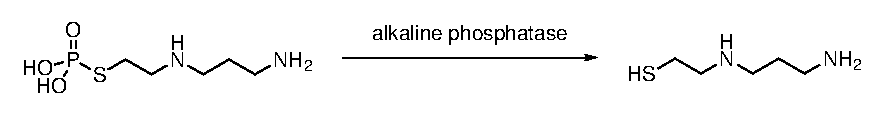
\includegraphics[scale=0.74]{Figures/amifostine.eps}
\caption{Amifostine, and its active metabolite.}\label{fig:amifostine}
\end{figure}

Despite the clear and serious side effects of radiotherapy, there is currently only one radioprotective pharmaceutical licensed by the FDA for use as such.
Amifostine (\cref{fig:amifostine}) is administered as a prodrug, which is phosphorylated \emph{in vivo} by alkaline phosphatase to form the free thiol which is able to scavenge radicals formed by irradiation.
Selectivity for healthy cells ultimately stems from the hypoxic nature of cancer cells, which inhibits dephosphorylation to the active compound\autocite{Kouvaris2007}.
However, due to the need for it to be present in relatively high concentration in the cytosol to effectively scavenge radicals, large doses are required, and this magnifies issues of cytotoxicity.
A more targeted approach is therefore required for effective radioprotection and a larger therapeutic window.

\subsection{Minor groove binding}
DNA is known to exist in many different structures (A-, B-, C-DNA etc.), depending on factors such as solvation and the presence of metal ions.
B-DNA, however, is by far the most prevalent in cells\autocite{Miyahara2012}.
The familiar double helix of B-DNA forms a major and a minor groove on either side of the sugar-phosphate backbone, where the nitrogenous bases are exposed.
There exists a class of small molecules which bind to this minor groove, and impart some property to the bound DNA.\@

The Hoechst stains, first synthesised in the early 1970s by the company \emph{Hoechst Aktiengesellschaft} as anthelmintic agents, are prototypical minor groove binders.
As can be seen in scheme \cref{fig:hoechst}, the gentle curvature of the molecule allows it to follow the DNA helix.
The benzimidazole moieties provide H-bond donors, which interact with acceptors in adenine and thymine.
At physiological pH, the molecule is positively charged, allowing further stabilisation of the DNA-Hoechst complex via electrostatic interactions with the electron rich sugar-phosphate backbone\autocite{Teng1988}.
The conjugated aromatic system imparts a strong UV absorbance at around \SI{350}{\nm}. Fluorescence in the visible spectrum is also observed, giving Hoechst compounds utility as DNA stains.

\begin{figure}
\centering
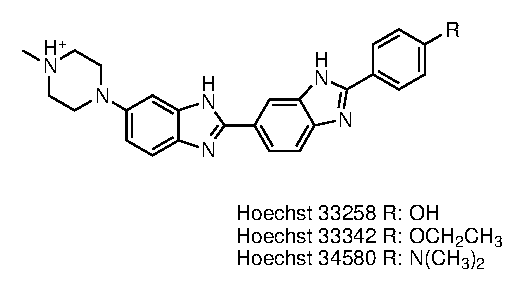
\includegraphics[scale=0.74]{Figures/hoechst.eps}
\caption{Hoechst stains, featuring the characteristic bis-benzimidazole motif.}\label{fig:hoechst}
\end{figure}

\subsection{Bis-benzimidazole derived radioprotectors}

In collaboration with the Peter MacCallum Cancer Centre, the White group has investigated a range of minor groove binders inspired by the Hoechst stains.
Methylproamine is a lead compound evaluated for radioprotection.
It was found to effectively protect cells from $\gamma$ and x-ray radiation, based on a clonogenic survival assay.
Pulse radiolysis studies suggested that the mechanism (for directly targeted cells) is based on direct repair of oxidative lesions, as opposed to scavenging ROS like amifostine.
When a DNA base (usually guanine) is ionised, a ``hole'' in the DNA is created.
This can be effectively transported along the length of the DNA molecule\autocite{Giese2002}.
The bound ligand (methylproamine) can then act as a reducing agent and neutralise the hole.

\begin{figure}
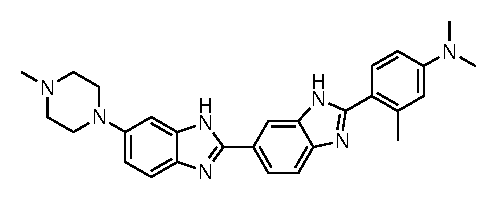
\includegraphics[scale=0.74]{Figures/methylproamine.eps}
\caption{Methylproamine, a lead compound identified for radioprotection.}\label{fig:methylproamine}
\end{figure}

\begin{figure}
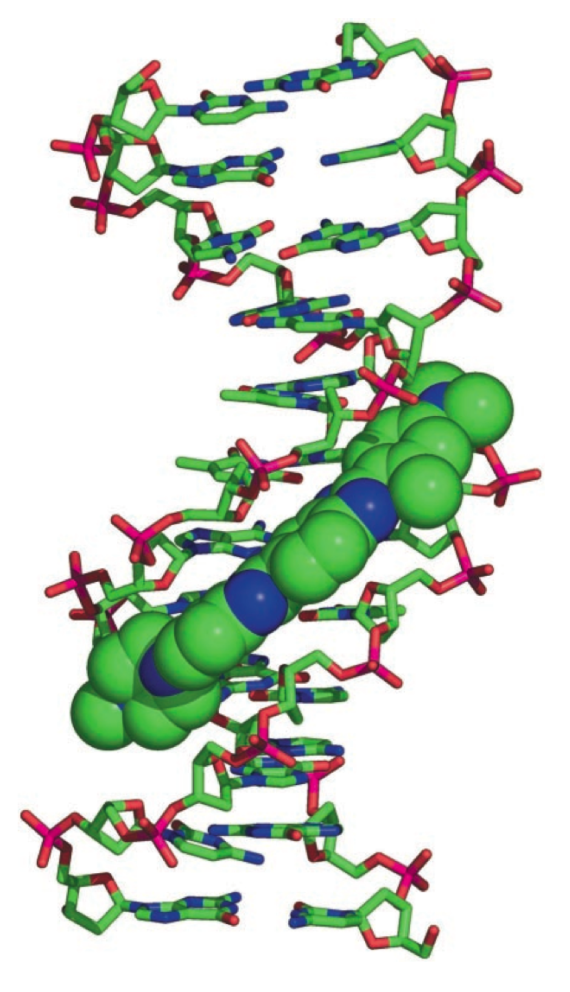
\includegraphics[width=0.3\textwidth]{Figures/mpa-dna-crystal.png}
\caption{Single crystal structure of methylproamine complexed with an AT rich DNA oligomer.}\label{fig:mpa-dna-crystal}
\end{figure}

\subsection{Proton-coupled electron transfer (PCET)}
The reduction mechanism of methylproamine and other bis-benzimidazole compounds is thought to be a proton-coupled electron transfer, in which an electron and proton are transferred from the ligand to the DNA in a stepwise process.
This was based on QSAR studies of a wide range of derivatives\autocite{Kakkar2005}.
It was found that the radioprotective potential was proportional to the acidity of the first benzimidazole proton.
This observation led to a new generation of radioprotectors with a 2-pyridyl group capping the first benzimidazole.
The lone pair of the pyridine nitrogen is able to donate into the $\sigma^{\star}$(\ce{N-H}) anti-bonding orbital and weaken the bond, allowing the proton to be more easily abstracted.

Substituting the N-methyl piperazinyl group for a N-morpholino group further improved the radioprotective ability of the bis-benzimidazole.
\emph{Ab initio} modelling showed the HOMO was centred around the lone pair of the morpholine nitrogen, and x-ray crystallography indicated that, when complexed with DNA, this lone pair pointed into the minor groove in an acceptable geometry for direct electron transfer.
The lead compound M2PB \cmpd{m2pb} was therefore synthesised, and showed very promising radioprotective ability, albeit with a relatively small therapeutic window.

\begin{figure}
\replacecmpd{m2pb}
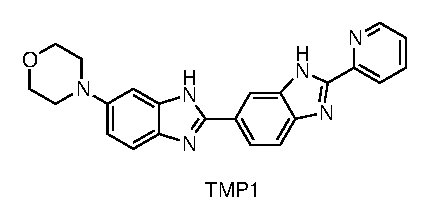
\includegraphics[scale=0.74]{Figures/m2pb.eps}
\caption{M2PB \refcmpd{m2pb}, an optimised lead compound for radioprotection.}\label{fig:m2pb}
\end{figure}


\subsection{Chalcogens as nitrogen bioisosteres}
Heavier group VI elements such as sulfur and selenium have been observed to behave similarly to nitrogen in biological systems.
A range of drugs have been developed that display this bioisosteric behaviour\autocite{Beno2015}.
The similarity between these elements is postulated to be due to the $\sigma$-hole that heavy main group elements exhibit, and their resulting propensity for Ch-bonding.

The fundamental aspects of Ch-bonding have been thoroughly discussed elsewhere in this thesis, suffice it to say that derivatives of the drug ebselen \cmpd{ebs} were identified early on as likely bioisosteres for a benzimidazole moiety.


\subsection{Ebselen as an antioxidant}\label{sec:simplification}
Ebselen itself, of course, displays antioxidant properties.
These are believed to be the basis for its neuroprotective, anti-helminthic, and anti-inflammatory behaviour.
The mechanism, however, appears to be completely different.
Ebselen behaves as a glutathione peroxidase mimic, that is to say, a catalyst that increases the rate at which glutathione reduces reactive oxygen species.

For this reason, we did not constrain ourselves to 2-pyridyl analogues (as the mechanism may not involve PCET), nor did we incorporate the morpholino substituent (as the HOMO is likely to be centred on the selenium).

\section{Synthesis of analogues}
\cmpd*{m2pb}
The initial target \cmpd{ebs-rhs-2py} were identified as likely minor groove binders, based on their similarity to the bis-benzimidazoles previously studied in the group (\cref{fig:dna-binding}).
Due to the difficulty of functionalising the benzisoselenazolinone system and the rationalisation in \cref{sec:simplification}, we simplified our targets to exclude the morpholino group.
We focussed on the synthesis of benzisoselenazolinone-benzimidazole \cmpd{ebs-rhs-2py}, as this appeared to be the most synthetically accessible using the chemistry developed in the group.

\begin{figure}
    \centering
    \replacecmpd{m2pb}
    \replacecmpd{ebs-rhs-2py}
    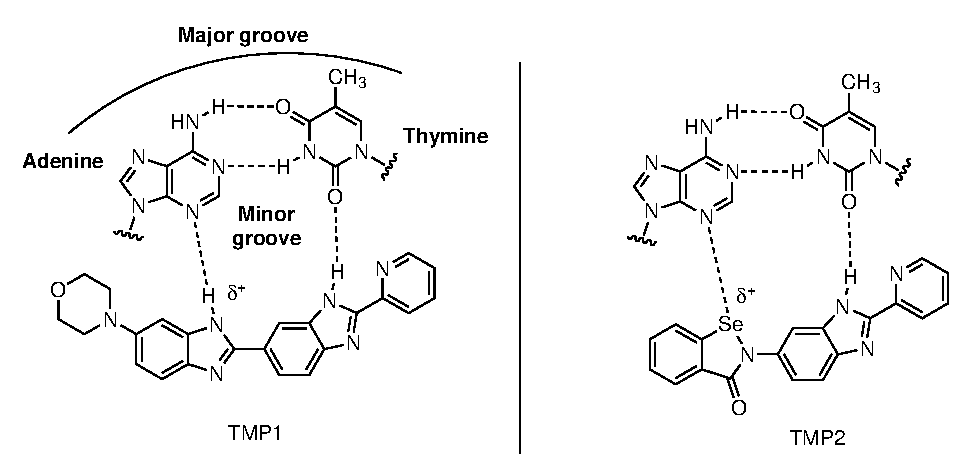
\includegraphics[scale=0.74]{Figures/dna-binding.eps}
    \caption{Schematic of DNA binding mode of benzimidazoles, and expected binding mode of a representative target.}\label{fig:dna-binding}
\end{figure}

\begin{comment}
\begin{figure}
    \centering
    \replacecmpd{m2pb}
    \replacecmpd{ebs-rhs-2py}
    \replacecmpd{ebs-ebs-2py}
    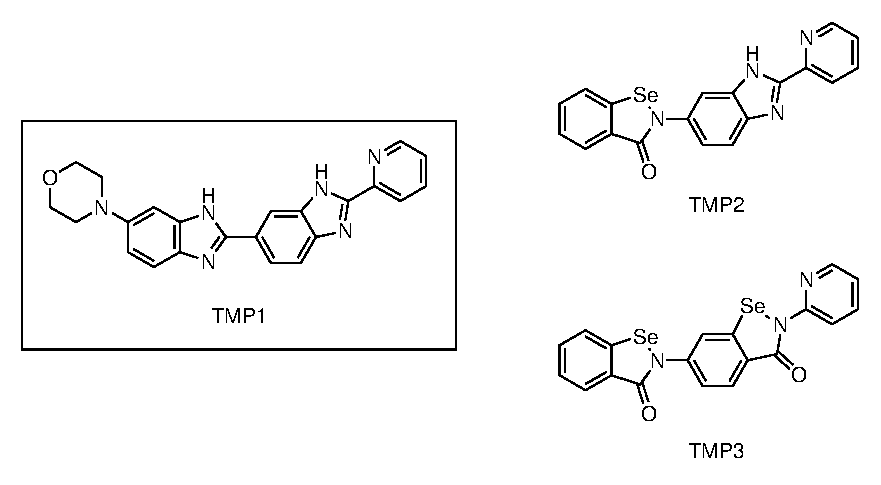
\includegraphics[scale=0.74]{Figures/targets.eps}
    \caption{Lead bis-benzimidazole \refcmpd{m2pb} and initial target compounds \refcmpd{ebs-rhs-2py,ebs-ebs-2py}.}\label{fig:targets}
\end{figure}
\end{comment}

\subsection{Preparation of benzisoselenazolinone-benzimidazole \refcmpd{ebs-rhs-2py}}

\subsubsection{Method 1: Ullmann coupling}\label{sec:carboximidate}

A number of routes to this compound were envisaged, via various intermediates.
Firstly, we were inspired by the Ullmann-type chemistry exploited by \citeauthor{Bhabak2010} in their selenocyclisation, and by the observation that the amidic proton in \cmpd{ebs.h} goes on to react further to furnish the tetracyclic compound \cmpd{tetracycle} (see \cref{ch:crystengcomm1})\autocite{Bhabak2010,Fellowes2019}.
We supposed that the intermediate \cmpd{ebs.h}, which can be prepared by reaction of the dichloride \cmpd{dichloride} with aqueous ammonia (\cref{sch:ebs-h-synthesis}) would be a suitable substrate for an Ullmann coupling with an aryl halide.
A number of test reactions were performed using the benzisothiazolinone \cmpd{ebs.h-thio}, which is commercially available and inexpensive.
Typical Ullmann conditions were used (high temperature, DMF solvent, high \ce{CuI} catalyst loading) to initially couple \cmpd{ebs.h-thio} with bromobenzene to afford \cmpd{ebs.thio} in moderate yield (\cref{sch:ebs-thio-ph-synthesis}).
We were also able to prepare ebselen \cmpd{ebs} via this route in similar yield.
Optimisation of the reaction was considered to be outside the scope of this work, so we proceeded with the synthesis of the bromo-benzimidazole coupling partner \cmpd{rhs-bromo-2py}.

\begin{scheme}
    \replacecmpd{dichloride}
    \replacecmpd{ebs.h}
    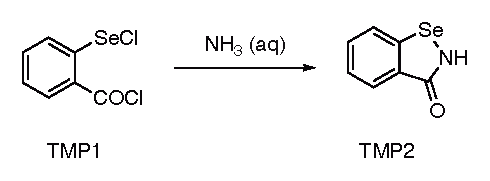
\includegraphics[scale=0.74]{Figures/ebs-h-synthesis.eps}
    \caption{Synthesis of \refcmpd{ebs.h}.}\label{sch:ebs-h-synthesis}
\end{scheme}

\begin{scheme}
    \replacecmpd{ebs.h,ebs.h-thio}
    \replacecmpd{ebs,ebs.thio}
    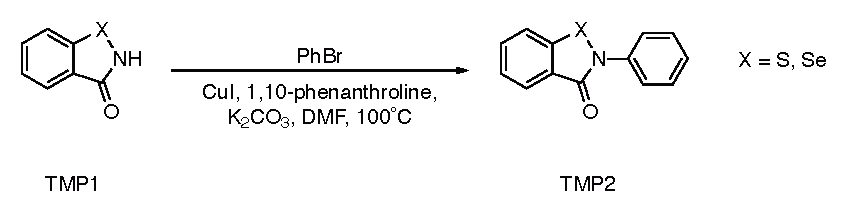
\includegraphics[scale=0.74]{Figures/ebs-thio-ph-synthesis.eps}
    \caption{Synthesis of \refcmpd{ebs} and \refcmpd{ebs.thio}.}\label{sch:ebs-thio-ph-synthesis}
\end{scheme}

4-bromo-2-nitroaniline was reduced to the diamine \cmpd{bromodiamine} using tin (II) chloride, then reacted with 2-pyridyl carboximidate hydrochloride \cmpd{2py-carboximidate} (prepared from 2-pyridyl carbonitrile) to afford the benzimidazole \cmpd{rhs-bromo-2py} in excellent yield.
Unfortunately this gave no detectable product in the coupling reaction.
We suspected that the benzimidazole proton may be competing with the amidic proton in the benzisothiazolinone ring, as it is substantially more acidic (pKa 16.4 vs $>20$), so we protected it using \emph{p}-methoxy benzyl chloride to give \cmpd[sub-counter-format=pg]{rhs-bromo-2py.pmb} (\cref{sch:rhs-protection}).
This afforded two distinct isomers from the two freely interconverting tautomers of \cmpd{rhs-bromo-2py}.
Although these were resolved by chromatography for subsequent reactions, this was likely not necessary, as deprotection would afford both tautomers.
Both isomers are therefore treated as a single compound here.

\begin{scheme}
    \replacecmpd{2py-carboximidate}
    \replacecmpd{bromodiamine}
    \replacecmpd{rhs-bromo-2py}
    \replacecmpd{rhs-bromo-2py.pmb}
    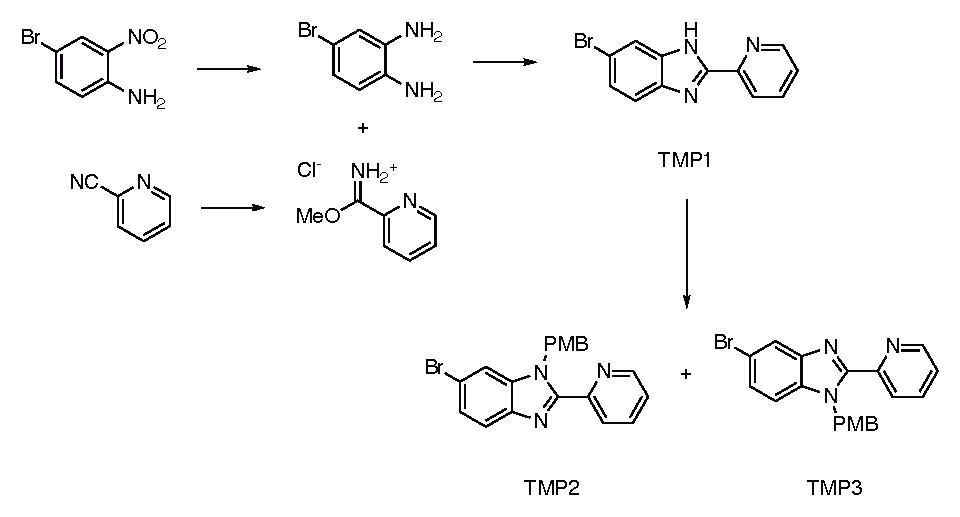
\includegraphics[scale=0.74]{Figures/rhs-protection.eps}
    \caption{Synthesis of \refcmpd{rhs-bromo-2py} and protection to form \refcmpd{rhs-bromo-2py.pmb}. (a) \ce{SnCl2.2H2O}, EtOH, reflux, 8~h, 92\%; (b) \ce{NaOMe}, MeOH, 80\degree{}C, 1~h; (c) MeOH, AcOH, reflux, 18~h, 91\%; (d) \ce{NaH}, PMBCl, DMF, 0\degree{}C $\rightarrow$ rt, 18~h, 82\%.}\label{sch:rhs-protection}
\end{scheme}

The PMB-protected benzimidazoles also gave no detectable coupling product, so we turned our attention to the catalyst/ligand system.
Ullmann couplings require a bidentate nitrogen-based ligand to coordinate the copper (I) species.
We used dimethylethylenediamine (DMEDA), although salicylates, 1,10-phenanthroline, 2,2\textprime-bipyridyl, tetramethylethylenediamine, and proline have also been used successfully in similar reactions.\autocite{Klapars2002,Altman2007,Sherborne2017}
The 2-(2-pyridyl)benzimidazole, even protected, resembles these ligands, and could reasonably be anticipated to coordinate the copper in competition with the ligand.
Although this does not necessarily preclude the coupling reaction, it does remove our ability to modify the coordination environment of the copper, to which the Ullmann reaction is very sensitive.
We attempted a ligand-free reaction to no avail, and thus concluded that the coordination environment of the copper is inappropriate for the reaction, and we would have to use another substrate.

We therefore prepared the phenyl derivative \cmpd{rhs-bromo-ph} via a metabisulfite coupling with benzaldehyde, and protected it similarly to give both isomers of \cmpd[sub-counter-format=pg]{rhs-bromo-ph.pmb}.
This gave the desired coupling product \cmpd*[sub-counter-format=pg]{ebs-rhs-ph.pmb}\cmpd[sub-counter-format=pg]{ebs-rhs-ph.thio-pmb} as a mixture of isomers, from one of which we obtained a single crystal structure (\cref{sch:ebs-thio-rhs-synthesis} and \cref{fig:ebs-thio-rhs-pmb-xray}).
Unfortunately, all efforts to deprotect the benzimidazole nitrogen failed.
A number of other protecting groups were trialled, including trityl, triphenylsilyl, \emph{t}-butyl and ethyl carbamates, however all either failed to give any protected product, or were too labile to survive the Ullmann reaction conditions.
We therefore abandoned this synthetic route.


\begin{scheme}
    \replacecmpd{ebs.h-thio}
    \replacecmpd{rhs-bromo-ph.pmb}
    \replacecmpd{ebs-rhs-ph.thio-pmb}
    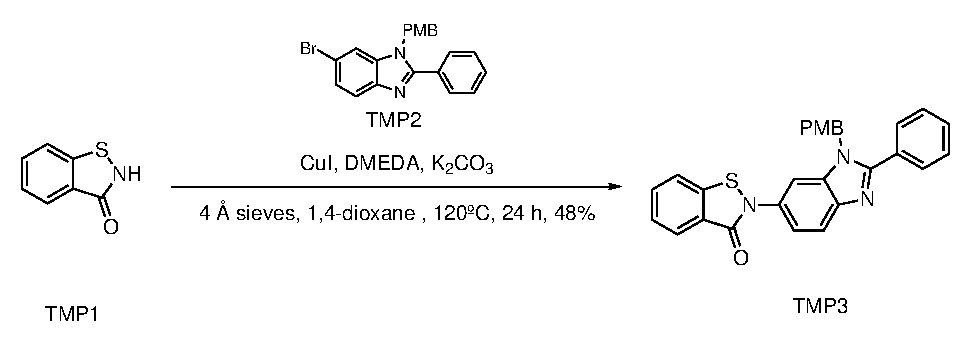
\includegraphics[scale=0.74]{Figures/ebs-thio-rhs-synthesis.eps}
    \caption{Synthesis of \refcmpd{ebs-rhs-ph.thio-pmb}.}\label{sch:ebs-thio-rhs-synthesis}
\end{scheme}

\begin{figure}
    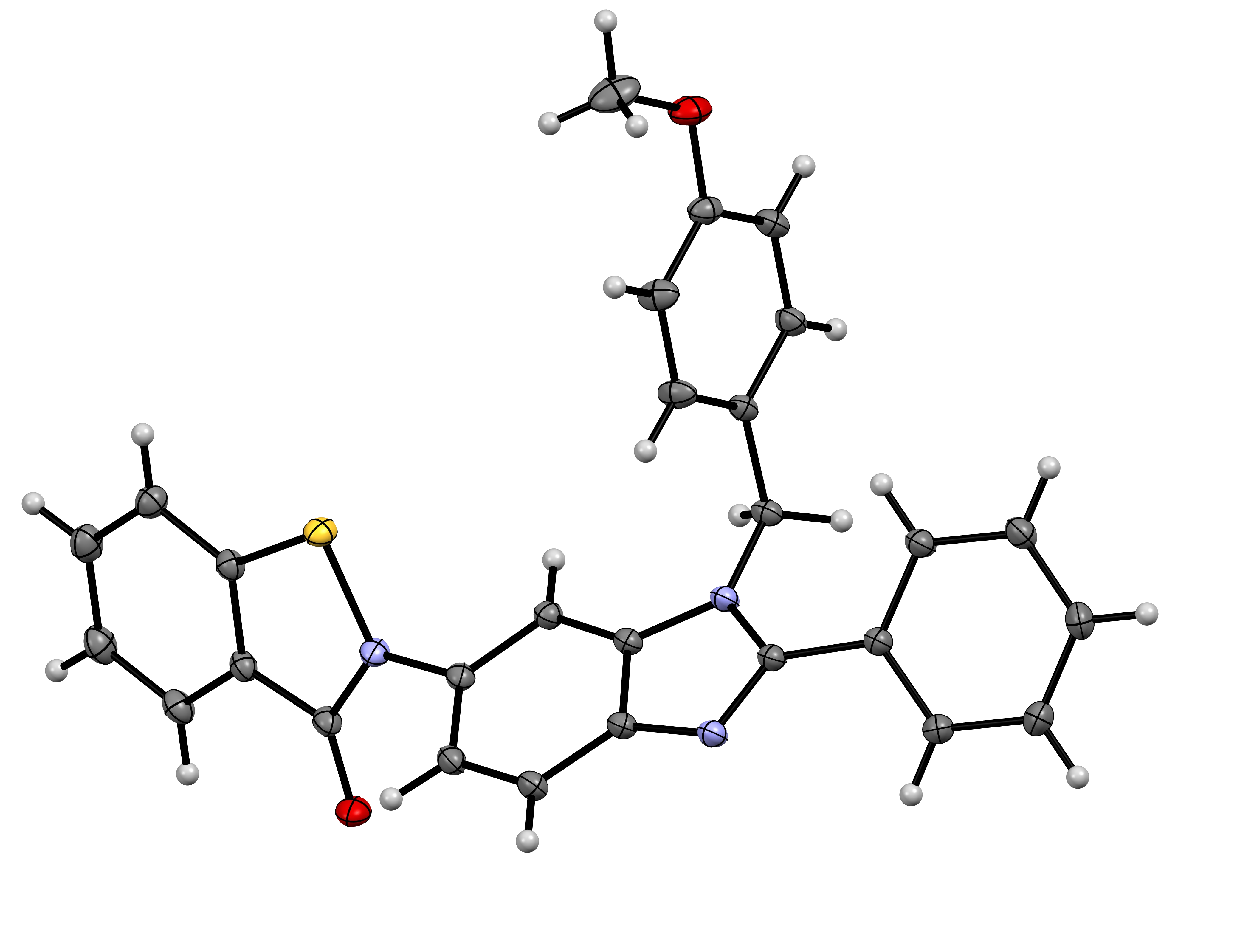
\includegraphics[width = 0.8\linewidth]{Figures/ebs-thio-rhs-pmb-xray.pdf}
    \caption{X-ray crystal structure of one isomer of \refcmpd{ebs-rhs-ph.thio-pmb}.}\label{fig:ebs-thio-rhs-pmb-xray}
\end{figure}

\subsubsection{Method 2: Benzisoselenazolinone-first route}\label{sec:reduction}

\begin{scheme}
    \replacecmpd{diselenide}
    \replacecmpd{dichloride}
    \replacecmpd{ebs-nitroaniline}
    \replacecmpd{ebs-nitroamide-2py}
    \replacecmpd{ebs-rhs-2py}
    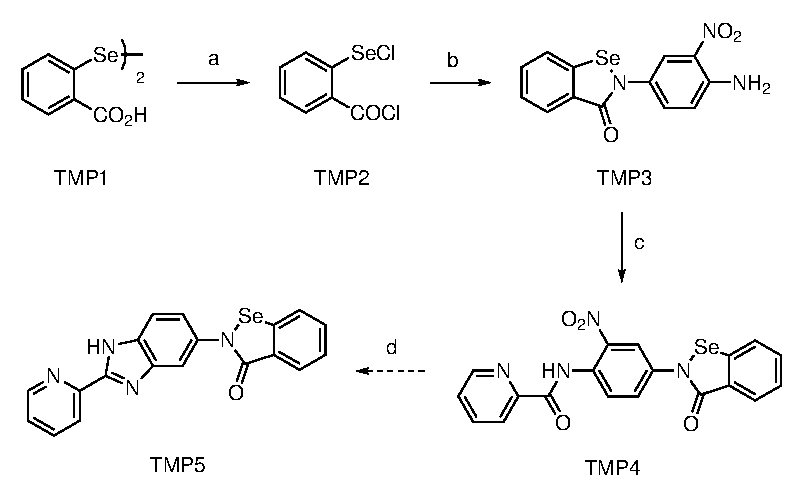
\includegraphics[scale=0.74]{Figures/ebs-synthesis3.eps}
    \caption[Proposed synthesis of \refcmpd{ebs-rhs-2py}]{Proposed synthesis of \refcmpd{ebs-rhs-2py}. (a) \ce{SOCl2}, cat. DMF, reflux, 30~min; (b) 2-nitro-1,4-benzenediamine, \ce{Et3N}, THF, rt, 18~h, 61\%; (c) Picolinic acid, TCBC, \ce{Et3N}, rt, 24~h, 20\%; (d) [H], \ce{H+}.}\label{sch:ebs-rhs-synthesis-1}
\end{scheme}

A revised route to this molecule is shown in \cref{sch:ebs-rhs-synthesis-1}, which involved first synthesising the benzisoselenazolinone moiety, then constructing the benzimidazole in a condensation and cyclisation.
The results of this, specifically the interesting crystal packing of the late stage intermediate \cmpd{ebs-nitroamide-2py} spurred the investigation detailed in \cref{ch:thermal-conversion}.
As this pathway did not involve copper catalysis, we reintroduced the 2-pyridyl group on the benzimidazole.
However, this route was not able to furnish the desired product, as the benzisoselenazolinone moiety did not tolerate the reduction conditions trialled.
Among the conditions trialled were:
\begin{itemize}
    \item palladium catalysed hydrogenation, from which we only recovered starting material presumably due to the catalyst being poisoned by the divalent selenium,
    \item tin (II) chloride/HCl reduction, which afforded a diselenide \cmpd{ebs-rhs-2py-diselenide} (\cref{fig:diselenide-benzimidazole-2py-xray}),
    \item dithionite reduction, which afforded a complex mixture of products.
\end{itemize}

\begin{figure}
    \centering
    \replacecmpd{ebs-rhs-2py-diselenide}
    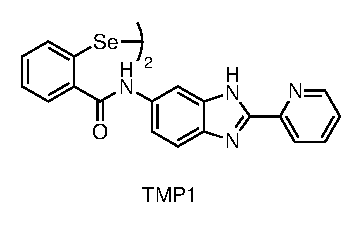
\includegraphics[scale=0.74]{Figures/ebs-rhs-diselenide.eps}

    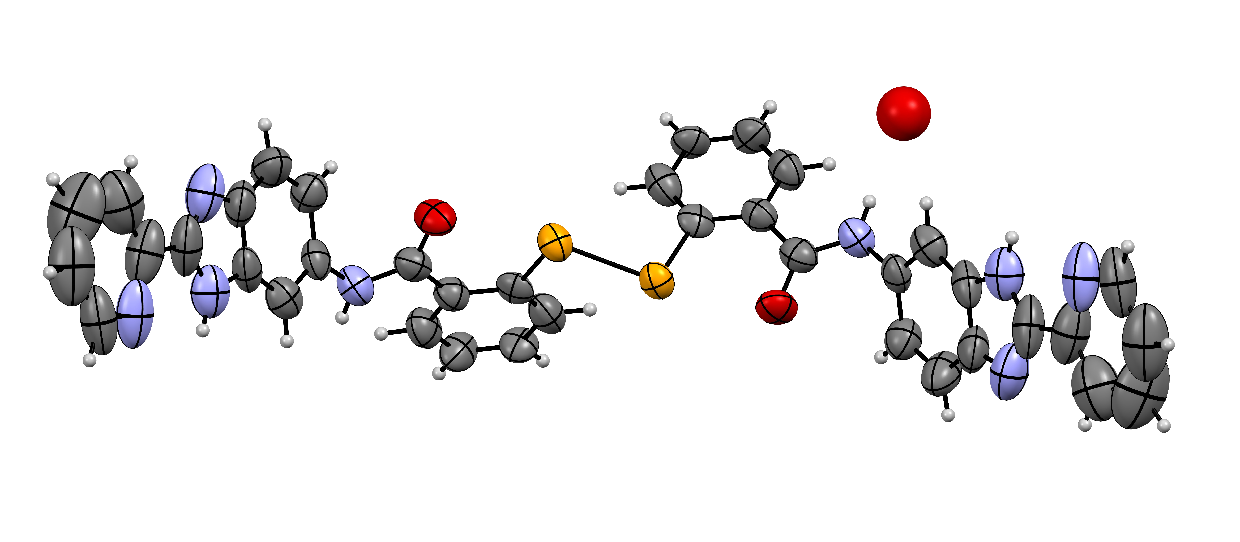
\includegraphics[width=0.8\linewidth]{Figures/diselenide-benzimidazole-2py-xray.pdf}
    \caption[X-ray crystal structure of \refcmpd{ebs-rhs-2py-diselenide}.]{X-ray crystal structure of \refcmpd{ebs-rhs-2py-diselenide} with a disordered water molecule.}\label{fig:diselenide-benzimidazole-2py-xray}
\end{figure}

\subsubsection{Method 3: Benzisoselenazoline-last route}

\begin{scheme}
    \replacecmpd{dichloride}
    \replacecmpd{rhs-nitro-amide}
    \replacecmpd{rhs-nitro}
    \replacecmpd{rhs-amine}
    \replacecmpd{ebs-rhs-ph}
    \caption[Synthesis of benzisoselenazolinone-benzimidazole Hoechst analogue \refcmpd{ebs-rhs-ph}.]{Synthesis of benzisoselenazolinone-benzimidazole Hoechst analogue \refcmpd{ebs-rhs-ph}. (a) BzCl, \ce{NEt3}, THF, rt, 18~h, 75\%; (b) \ce{BF3\cdot OEt2}, 1,4-dioxane, reflux, 3.5~h, 93\%; (c) \ce{SnCl2}, EtOH, reflux, 2~h, 87\%; (d) \refcmpd{dichloride}, MeCN, \ce{NEt3}, rt, 18~h, 8\%.}
    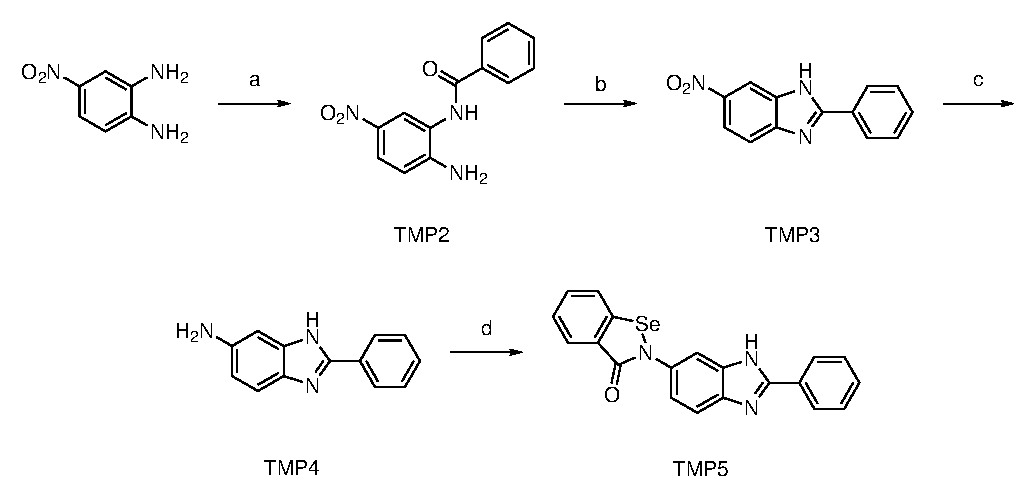
\includegraphics[scale=0.74]{Figures/ebs-rhs-synthesis.eps}\label{sch:ebs-rhs-synthesis-2}
\end{scheme}

We therefore devised another scheme in which the benzisoselenazolinone ring is formed last, as the delicate nature of this group appeared to be hindering our efforts (\cref{sch:ebs-rhs-synthesis-2}).
This initially involved formation of an amide \cmpd{rhs-nitro-amide} by treating 3,4-diamino-1-nitrobenzene with an acid chloride.
It was found that the acid chloride of picolinic acid (which would ultimately afford the 2-(2-pyridyl) benzimidazole) was not stable, decomposing almost as soon as it was formed.
We investigated using the carboximidate as in \cref{sec:carboximidate}, however the nitro group on the diamine proved to be too deactivating; the aniline nitrogens were not sufficiently nucleophilic to react with the carboximidate.
Rather than investigate other pathways to this compound (such as the use of coupling agents), we again decided to simplify the system to a phenyl ring (to ultimately give \cmpd{ebs-rhs-ph}).
We therefore formed \cmpd{rhs-nitro-amide} using benzoyl chloride in excellent yield, which underwent cyclisation in the presence of the strong Lewis acid \ce{BF3\cdot OEt2} to form \cmpd{rhs-nitro}.
Tin (II) chloride reduction of the nitroarene \cmpd{rhs-nitro} afforded the aniline \cmpd{rhs-amine} as the hexachlorostannate salt.
This was coupled to the bis-electrophile \cmpd{dichloride} to afford the desired benzisoselenazolinone-benzimidazole \cmpd{ebs-rhs-ph}, which formed single crystals suitable for x-ray diffraction by slow evaporation from DMSO (\cref{fig:ebs-rhs-xray}).

\begin{figure}[ht]
    \centering
    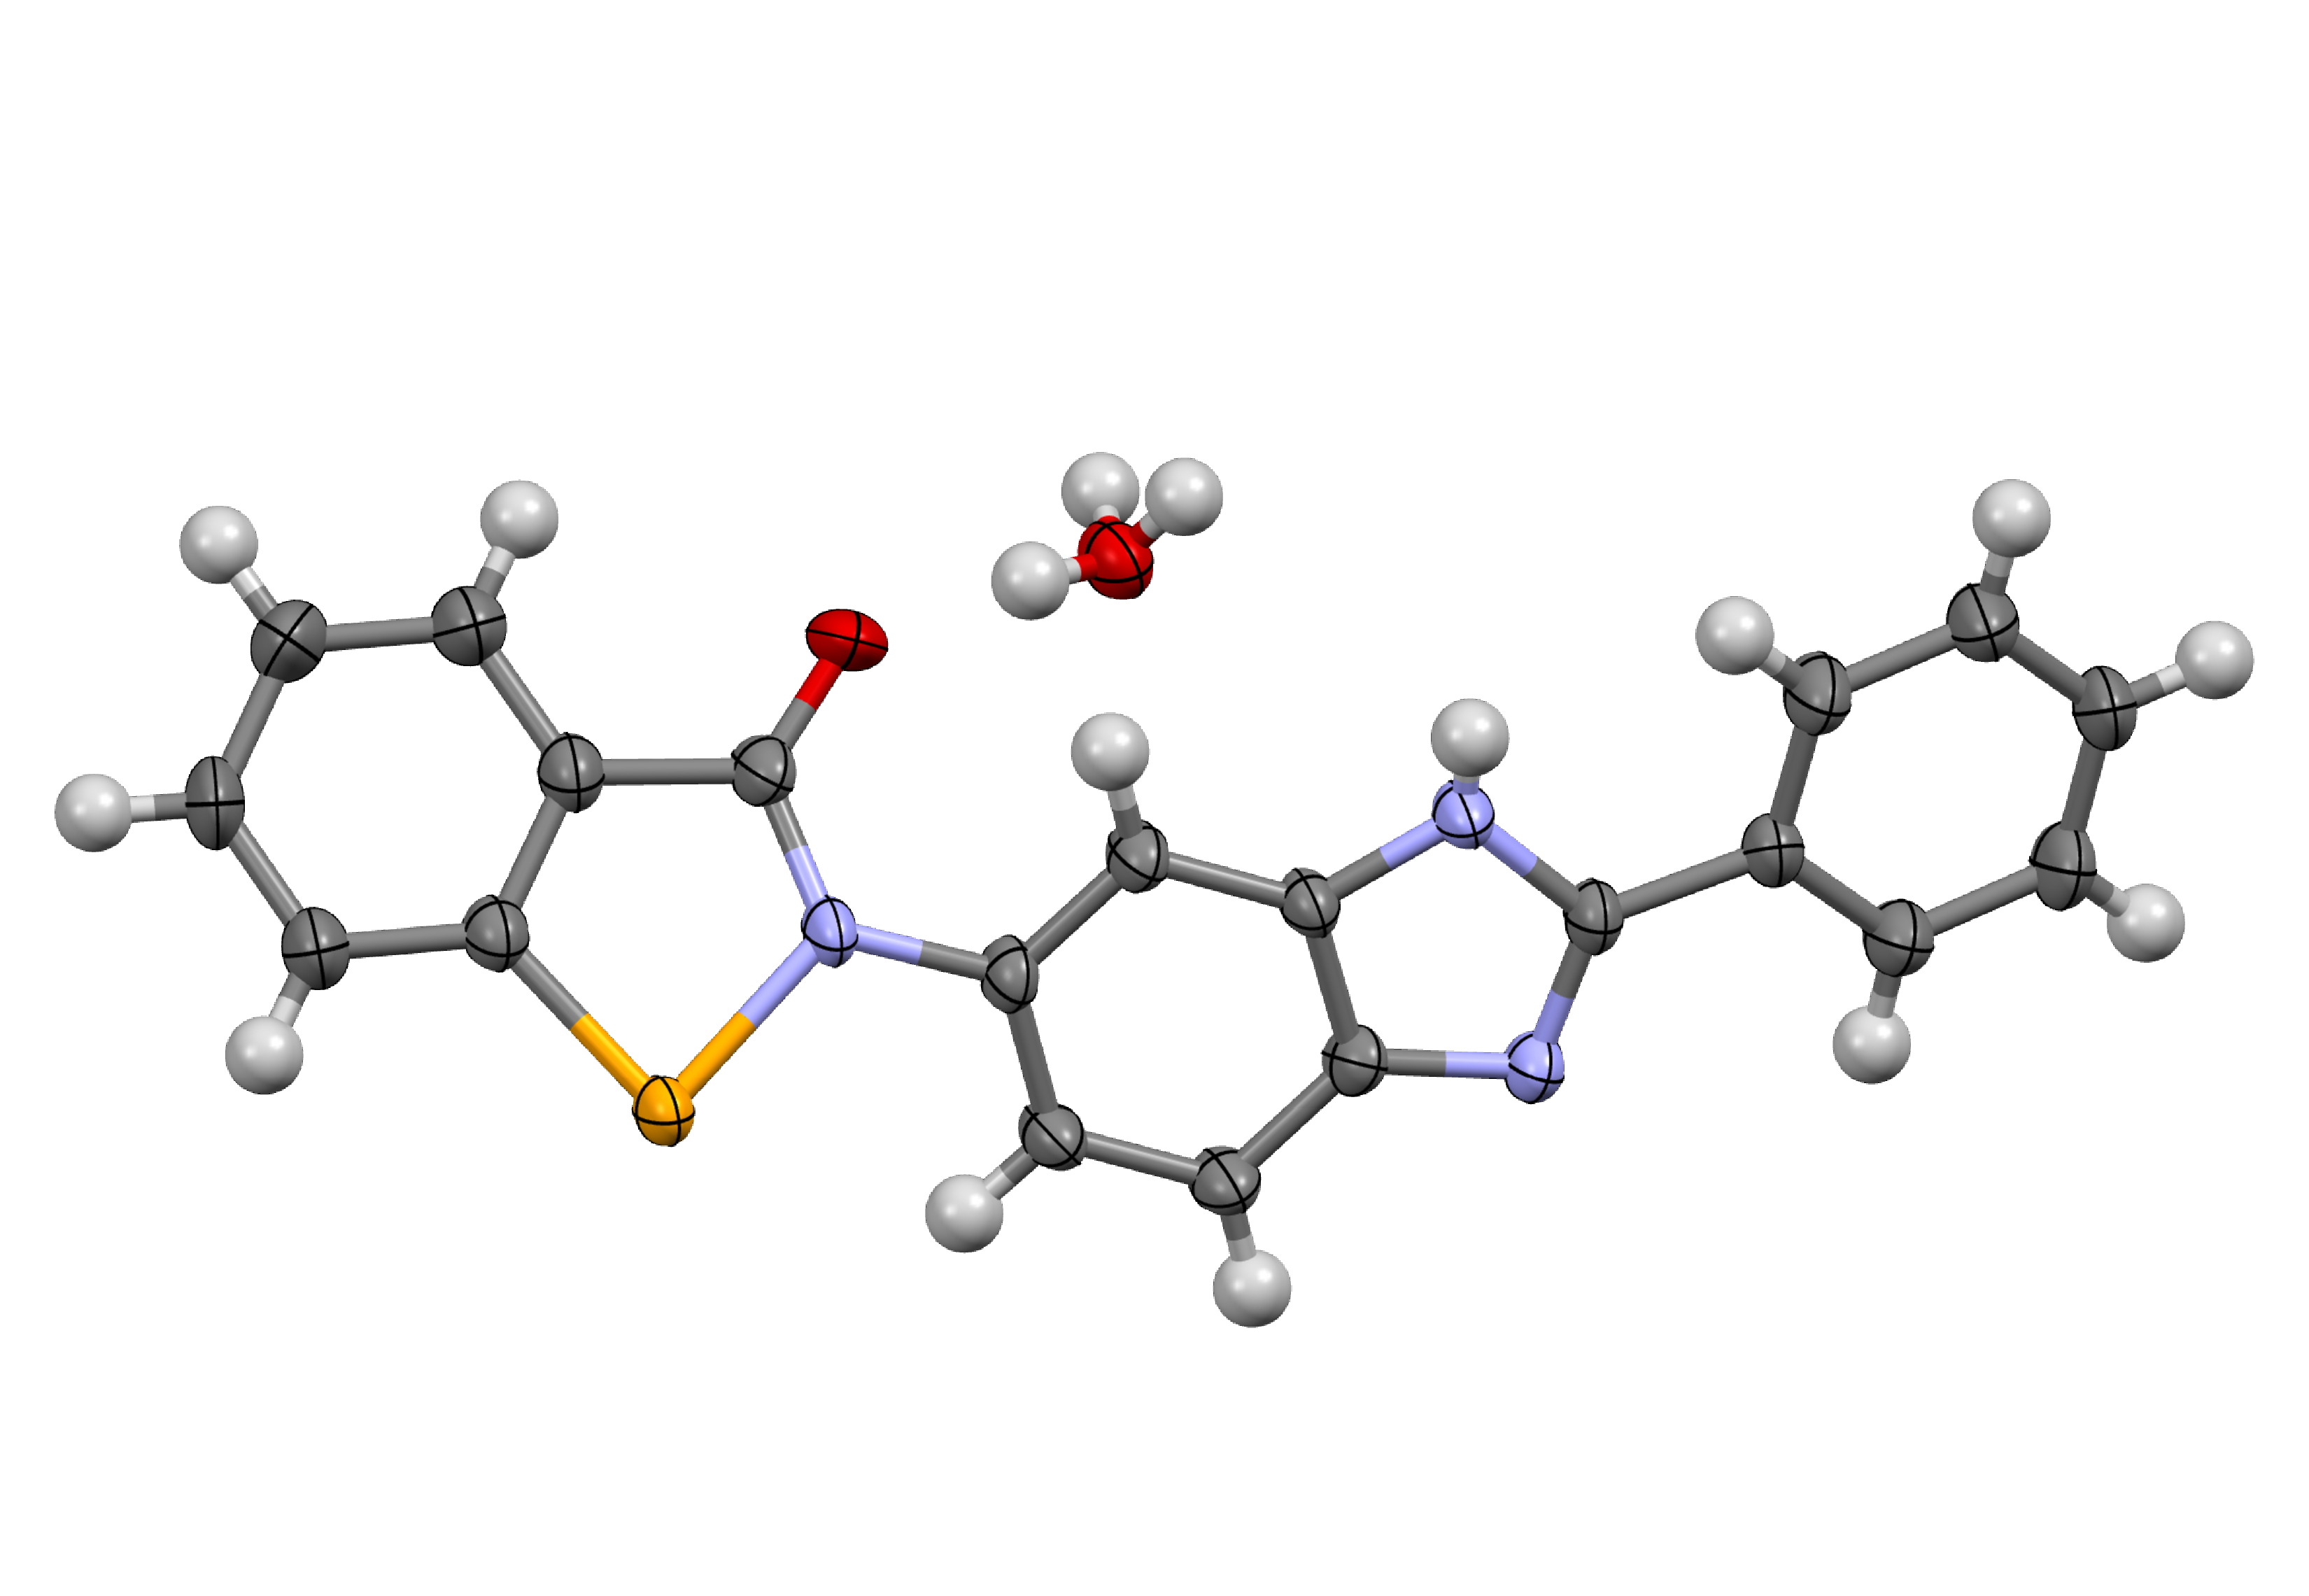
\includegraphics[width=0.8\linewidth]{Figures/ebs-rhs-xray.pdf}
    \caption[X-ray crystal structure of \refcmpd{ebs-rhs-ph}.]{X-ray crystal structure of \refcmpd{ebs-rhs-ph}. The water is disordered over 3 sites, with each proton having an occupancy of 2/3.}\label{fig:ebs-rhs-xray}
\end{figure}

\section{DNA binding studies}
Previous studies of Hoechst derivatives have shown that radioprotective ability is strongly correlated with a high affinity for the minor groove of DNA.\@
Although it is conceivable that ROS may be reduced in the cytoplasm by radioprotector molecules, this does not appear to be the major method of radioprotection for these compounds.

\subsection{Co-crystallisation results}
The main technique used to provide evidence of DNA binding is co-crystallisation of the ligand with DNA oligomers.
This can also provide detailed information on the specific mode of binding.
Unlike the co-crystallisation experiments used earlier in this thesis, this experiment bears more similarity to the techniques employed in macromolecular crystallisation, simply due to the delicate nature of the DNA oligomers.
Vapour diffusion from hanging drops was selected as the method for growing the crystals.
Hanging drop crystallisation relies on the equilibration of water between a reservoir of certain osmotic potential, and a droplet just above it containing the components of the crystal.
The main benefit is the slow rate of diffusion of water between the droplet and the reservoir, which leads to the formation of high quality crystals.
The technique is also quite efficient, in that only small amounts of compound are used.

The components of the drops were as follows:

\begin{itemize}
    \item DNA oligomer, the A2T2 self-complimentary 16mer was used for all experiments (CGCGCGAATTCGCGCG);
    \item ligand molecule \cmpd{ebs-rhs-ph};
    \item spermine hydrochloride, a polycationic tetramine which helps to stabilise the negative charge on the phosphate backbone of the DNA;\@
    \item \ce{MgCl2}, a source of \ce{Mg^{2+}} cations to further stabilise the negative DNA;\@
    \item sodium cacodylate, a buffer to ensure constant pH, and to inhibit microbial growth;
    \item water, the solvent;
    \item 2-methyl-2,4-pentanediol, the anti-solvent.
\end{itemize}

The solvent reservoir contained only water and 2-methyl-2,4-pentanediol.

Unfortunately, we were not able to obtain co-crystals of \cmpd{ebs-rhs-ph} with the DNA oligomer, as precipitation of an amorphous solid occurred upon addition of the ligand solution to the drop.
This suggested that solubility of the compound may be an issue, which is fairly common among bis-benzimidazoles.

In order to circumvent this, we instead grew crystals of the DNA oligomer in the absence of the ligand.
This afforded large crystals suitable for x-ray diffraction.
To introduce the ligand into the minor groove, we soaked the DNA crystals in a solution of the ligand in crystallisation buffer.
The DNA crystal structure contains substantial amounts of disordered water, forming channels through which the ligand may diffuse (\cref{fig:dna-oligo}).
However, upon exposure to the ligand, the DNA crystals appeared to disintegrate to give a similar amorphous precipitate.

We therefore abandoned this method of characterising the binding of the ligand.

\begin{figure}
    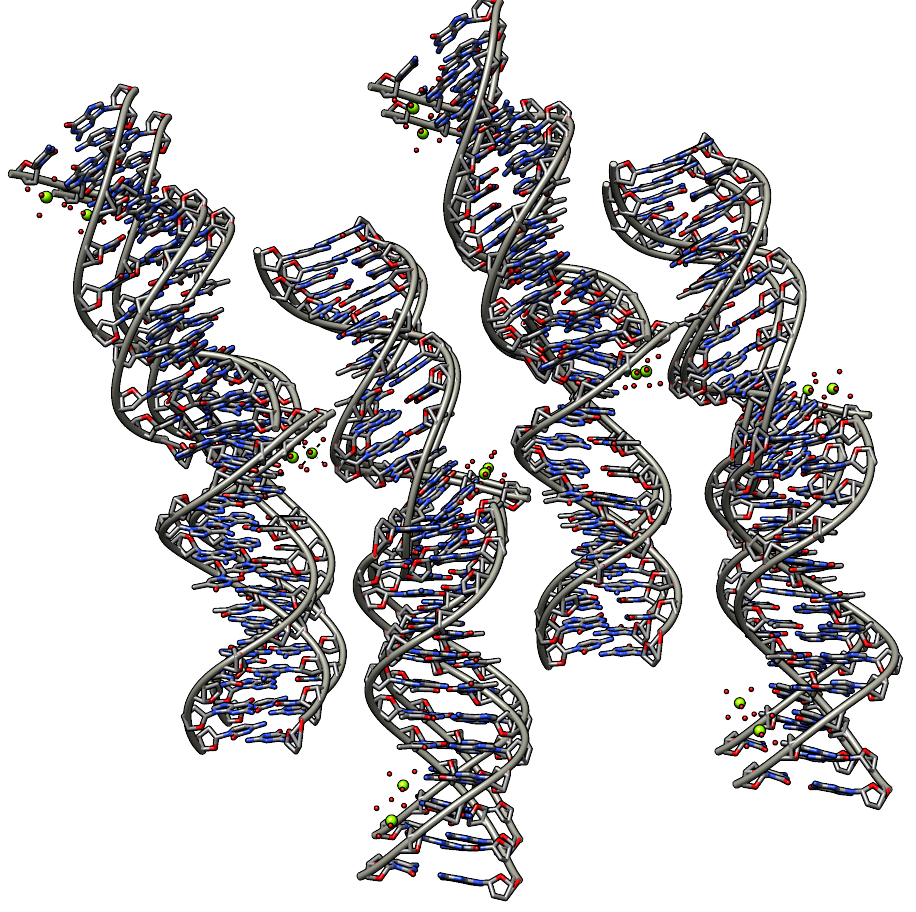
\includegraphics[width=0.7\linewidth]{Figures/dna_oligo.png}
    \caption{Crystal packing of the A2T2 self-complimentary DNA 16mer, showing the open channels between the DNA molecules.}\label{fig:dna-oligo}
\end{figure}

\subsection{UV-Vis titration}\label{sec:absorbance}
In the absence of a co-crystal structure, we sought to measure the binding of the ligand by UV-Vis titration.
Briefly, this works by measuring the degree of conjugation between the two benzimidazole (or benzimidazole-like) systems.
Free bis-benzimidazoles have a significant torsion about the central bond.
This leads to relatively poor orbital overlap and conjugation between the benzimidazoles, and an associated blue shift in the absorbance spectrum as compared to a completely planar molecule of the same size.
As the bis-benzimidazole binds to the minor groove of a DNA molecule, a more planar geometry is imposed, so the orbital overlap is improved and the absorbance peak moves towards the red.
By the application of a simple binding model, a dissociation constant can be derived.

Also visible in these titration experiments are spectroscopic signatures of different types of binding, including intercalation and major groove binding.
Both of these are referred to as non-specific binding, as they do not rely on the presence of four consecutive A-T pairs to expose H-bond acceptors in the minor groove.
These types of binding are not associated with a bathychromic shift in the absorbance spectrum, but instead with a quenching of the signal.
It is important to note that non-specific binding occurs simultaneously with specific minor groove binding, but the latter, when present, dominates the changes in the absorbance spectrum.

In order to assess the binding constant, the absorption spectrum and extinction coefficient for the free ligand must be measured.
The extinction coefficient at $\lambda_{\text{max}} = 309$~nm for \cmpd{ebs-rhs-ph} in 0.1\% TFA/45\% MeOH was determined to be 21062~M$^{-1}$cm$^{-1}$ (\cref{fig:ebs-rhs-ph-calcurve}).

\begin{figure}
    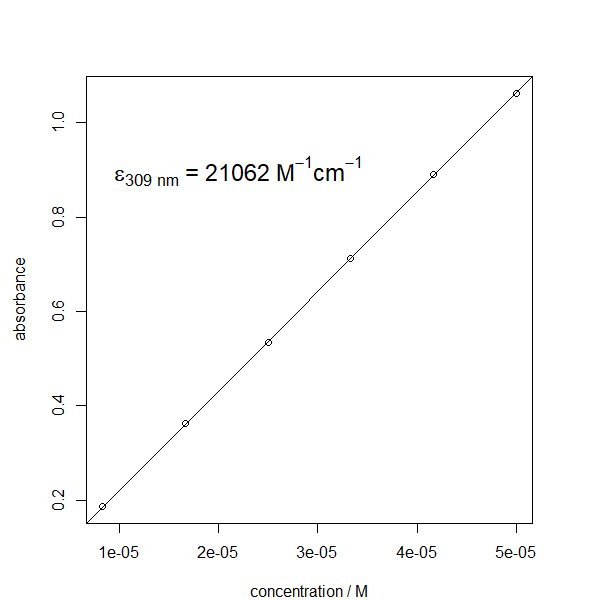
\includegraphics[width=0.5\linewidth]{Figures/ebshoe-calibration.png}
    \caption{Calibration curve for \refcmpd{ebs-rhs-ph}.}\label{fig:ebs-rhs-ph-calcurve}
\end{figure}

The titration was then carried out using a solution of the ligand in 0.1\% TFA/45\% MeOH (15~$\mu$M) and diluted DNA stock (0.025~mMbp), and the resulting spectra are shown in \cref{fig:ebshoe-ctdna-lowconc}.
A shift in absorbance is not readily apparent at such low DNA concentrations, so the experiment was repeated using 2~mMbp DNA stock, and the resulting spectra are shown in \cref{fig:ebshoe-ctdna-hiconc}.
At this concentration, we observed precipitation of the ligand and DNA, which can be seen in the broadly absorbing tail in the spectra.
This is highly undesirable, as the resulting data cannot be used to calculate the binding affinity.

\begin{figure}
    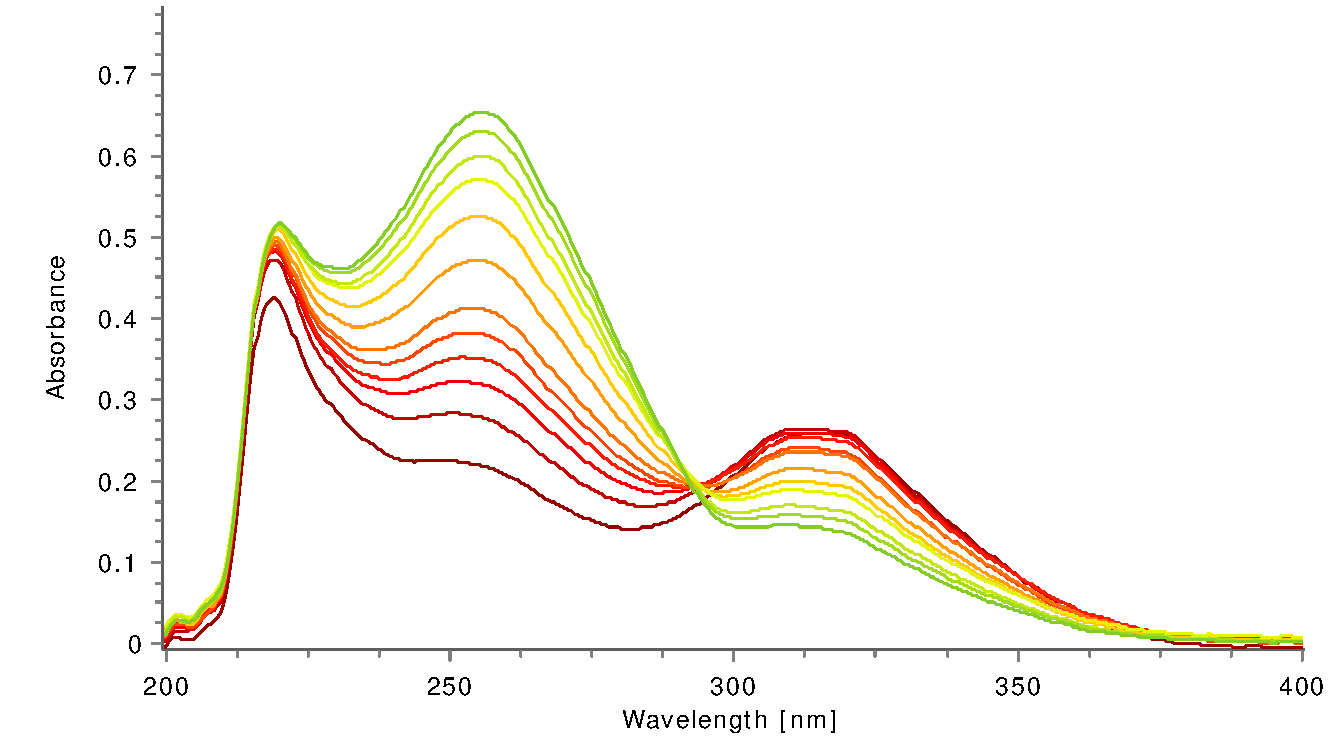
\includegraphics[width=0.7\linewidth]{Figures/ebshoe-ctdna-lowconc.pdf}
    \caption{UV-vis titration of \refcmpd{ebs-rhs-ph} with ct-DNA at low DNA stock concentration.}\label{fig:ebshoe-ctdna-lowconc}
\end{figure}

\begin{figure}
    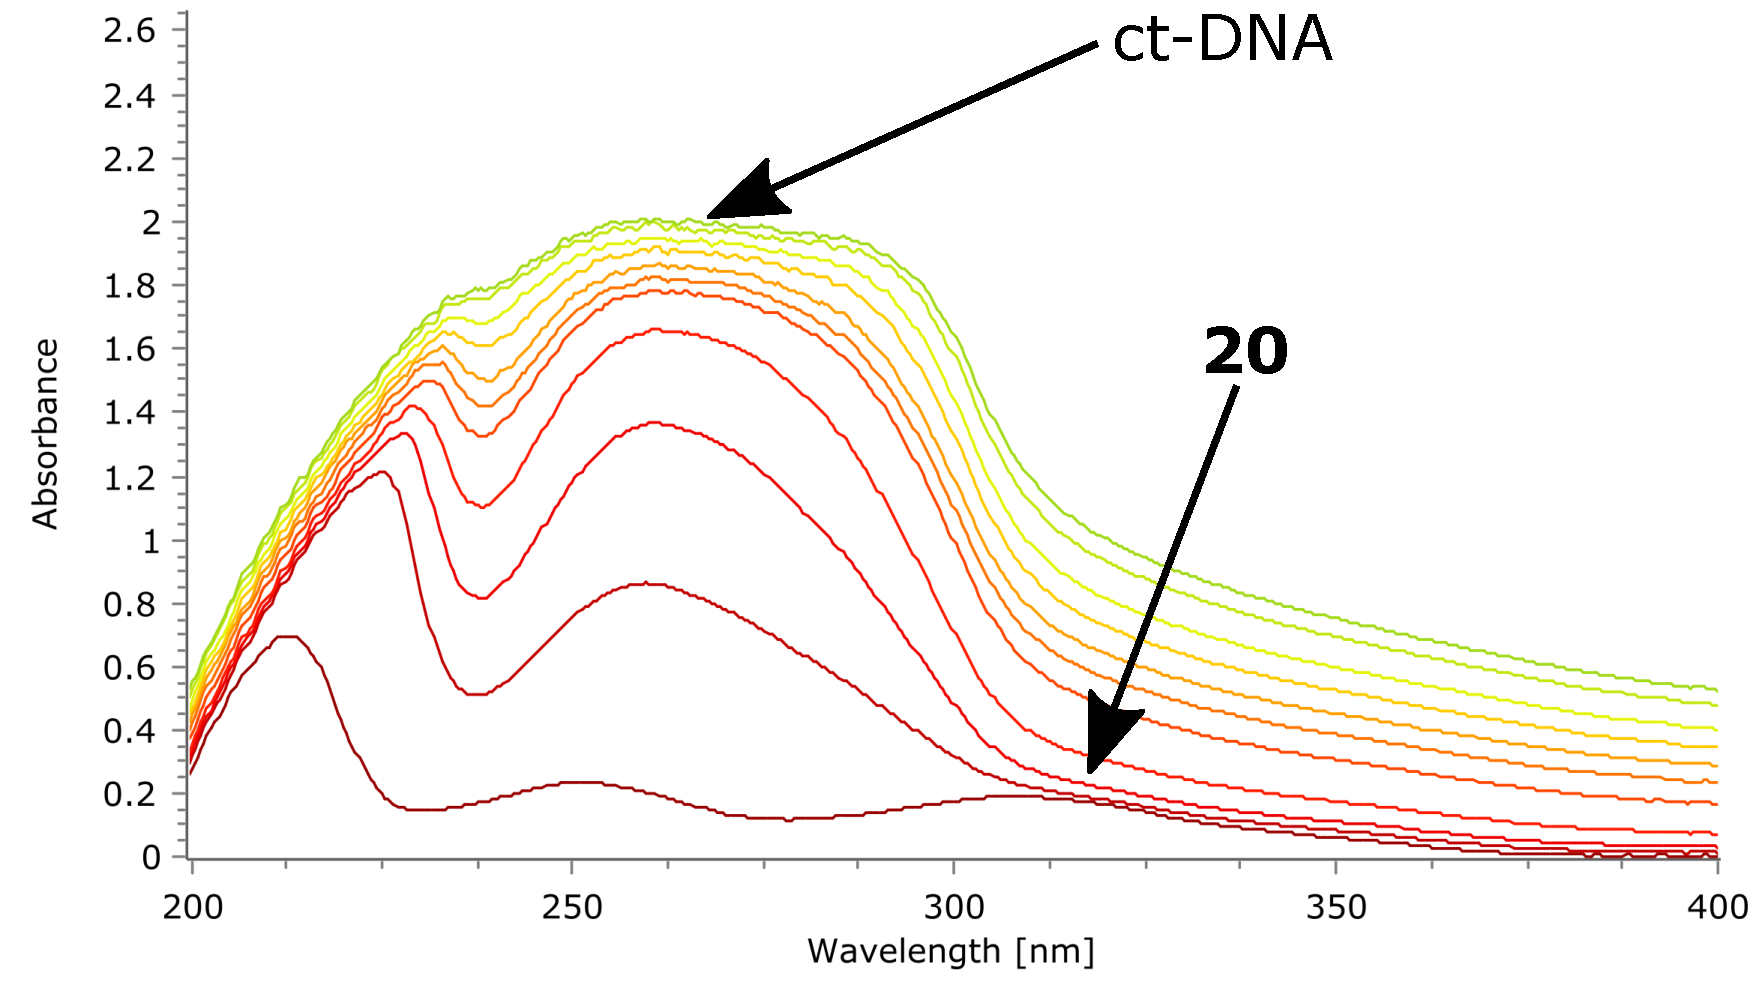
\includegraphics[width=0.7\linewidth]{Figures/ebshoe-ctdna-hiconc.pdf}
    \caption{UV-vis titration of \refcmpd{ebs-rhs-ph} with ct-DNA at high DNA stock concentration.}\label{fig:ebshoe-ctdna-hiconc}
\end{figure}

A further sample of the precipitate was prepared using the same conditions, and the solid isolated by centrifuging.
The supernatant was pipetted off, and the UV-vis spectrum revealed no absorbance at 309~nm, so we concluded that all of the ligand was contained in the precipitate.
The solid was washed with T/E/N buffer (\footnote{20~mM TRIS, pH 7.2; 1~mM EDTA\ce{\cdot 2 Na^+}; 100~mM \ce{NaCl}; 10\% v/v DMSO}) to remove excess DNA, and 0.1\% TFA/45\% MeOH to remove excess ligand, dried in vacuo, then dissolved in \ce{\textit{d}6}-DMSO.\@
\ce{^{1}H}-NMR revealed that the solid contained nucleic acid material (in the downfield region) as well as aromatic signals consistent with the ligand (\cref{fig:ebshoe-dna-adduct}).
We suspected that this was the same amorphous material that formed in the co-crystallisation experiment, and attribute its formation to a reaction between the ligand and the DNA.\@

\begin{figure}
    \centering
    \begin{subfigure}{\linewidth}
        \centering
        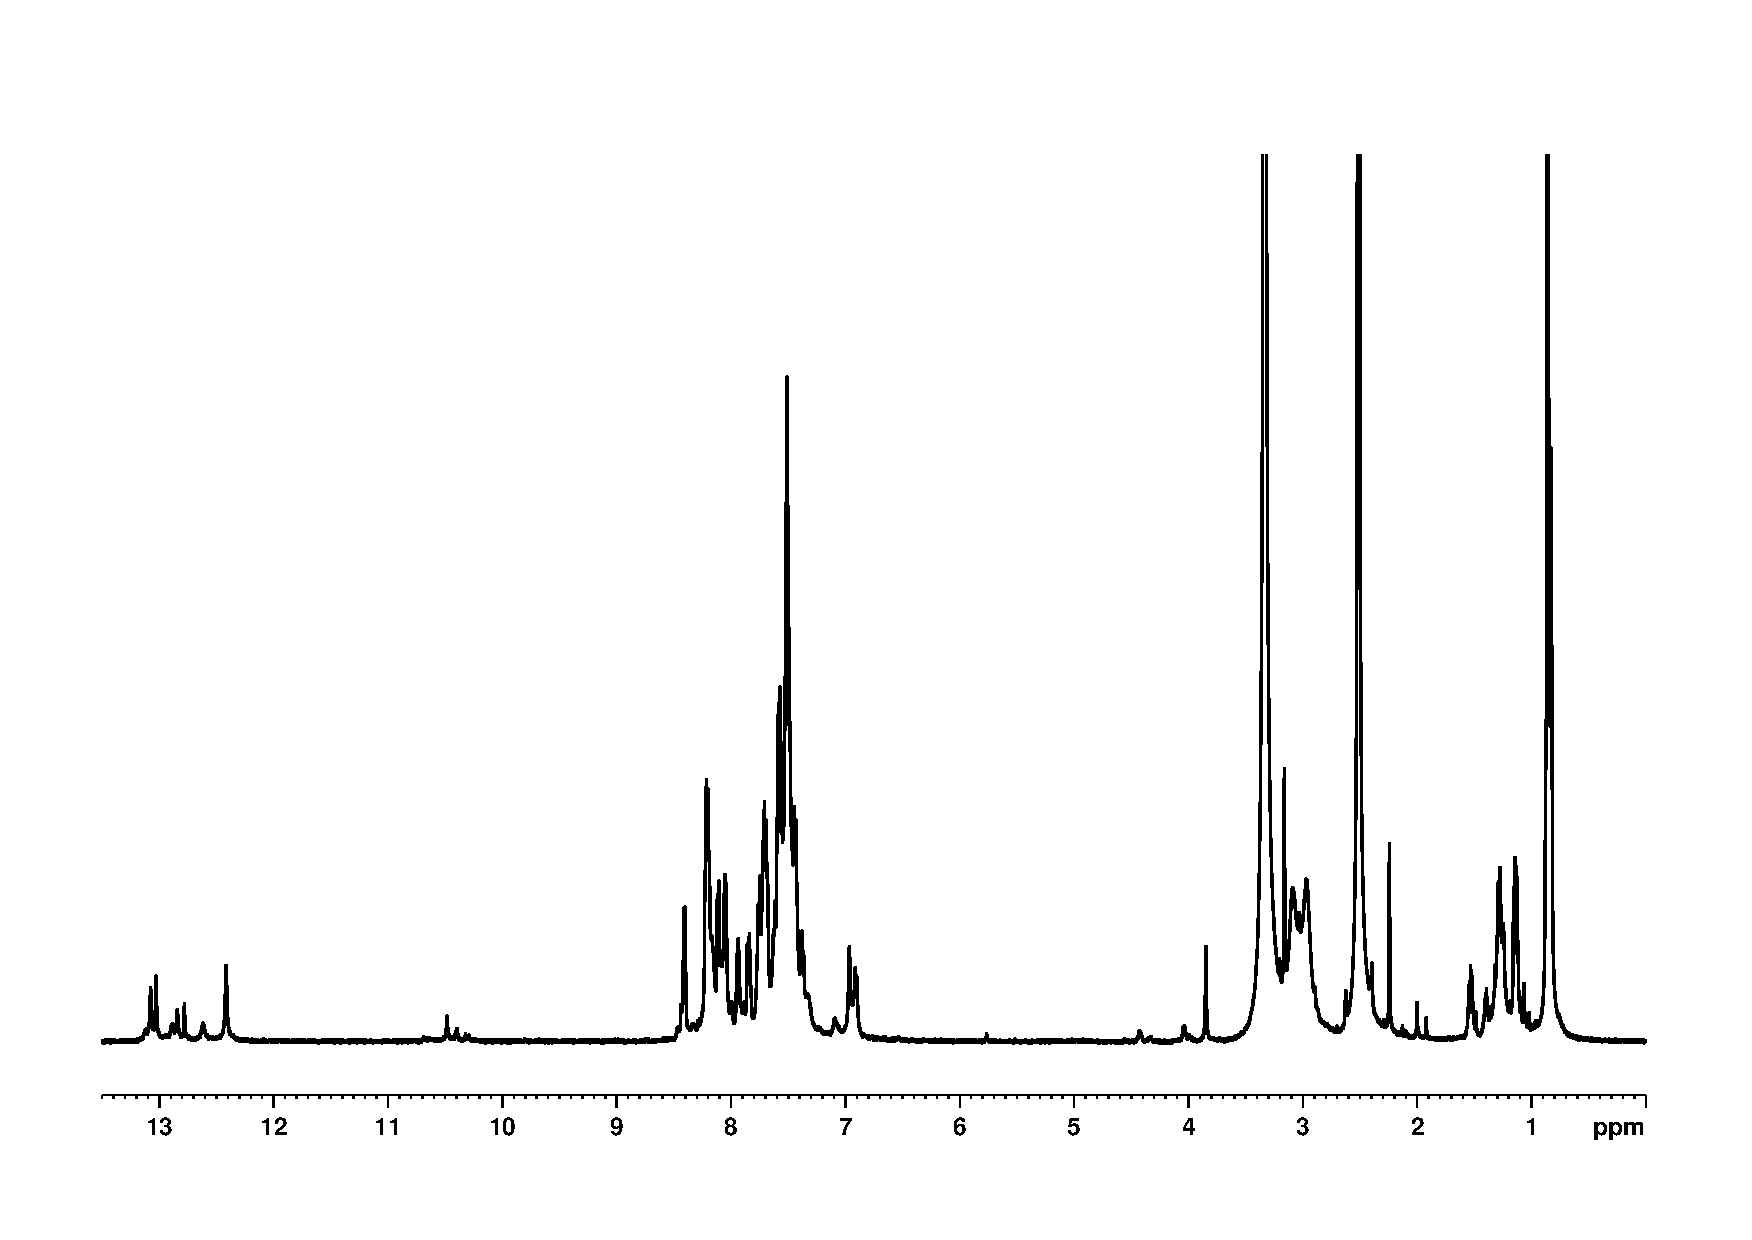
\includegraphics[width=0.8\linewidth]{Figures/ebshoe-dna-adduct-full.pdf}
        \caption{}
    \end{subfigure}
    \begin{subfigure}{\linewidth}
        \centering
        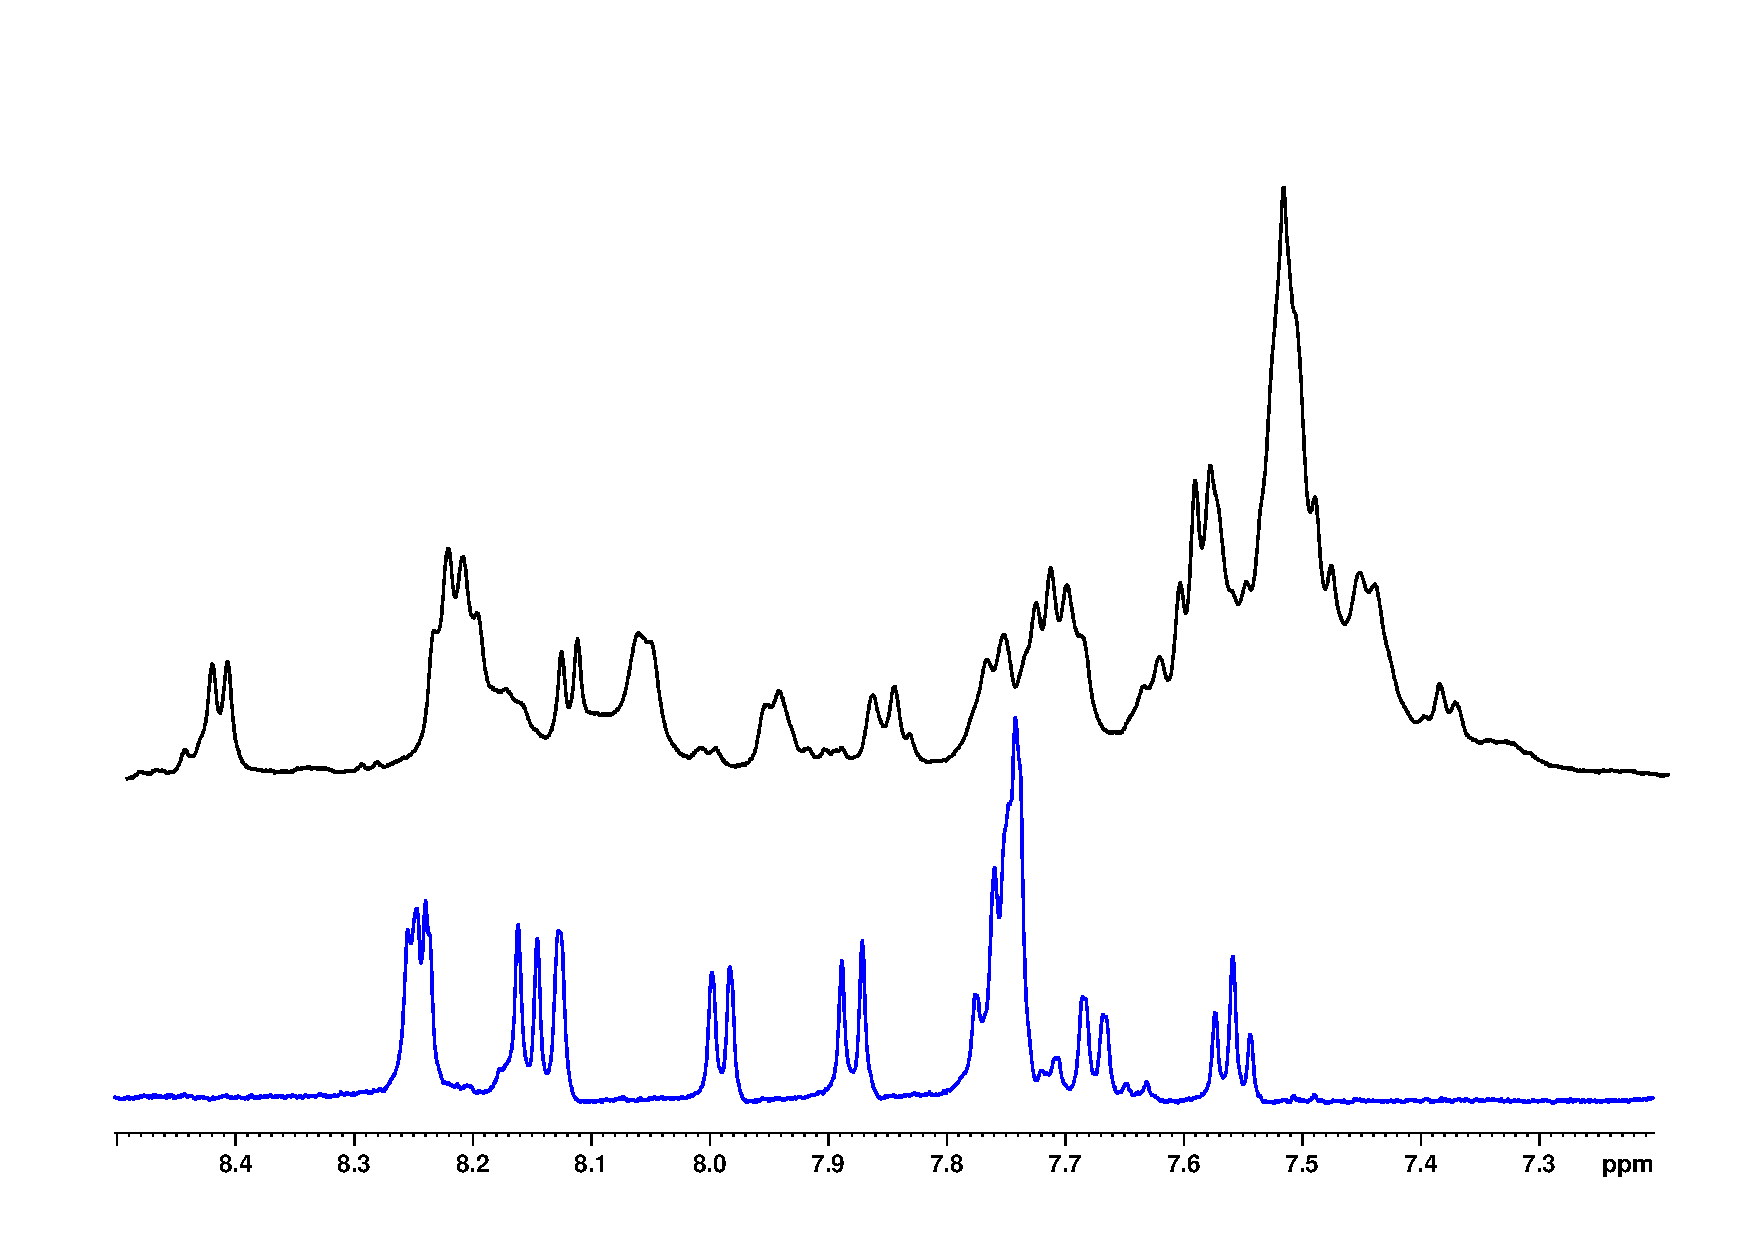
\includegraphics[width=0.8\linewidth]{Figures/ebshoe-dna-adduct-aromatic.pdf}
        \caption{}
    \end{subfigure}
    \caption{\ce{^{1}H}-NMR spectra of the adduct of \refcmpd{ebs-rhs-ph} with ct-DNA, and the pure ligand (blue) for comparison.}\label{fig:ebshoe-dna-adduct}

\end{figure}

Ebselen is known to form covalent adducts with many biomolecules.
Indeed, the covalent complex with glutathione is responsible for its antioxidant properties.\autocite{Antony2011}
Its activity against an number of other targets (e.g.\ superoxide dismutase\autocite{Capper2018}) is mediated through reactions with cysteine residues, so the formation of a covalent complex with DNA is perhaps not surprising.
Unfortunately this makes \cmpd{ebs-rhs-ph} useless for the radioprotectors project, as a core requirement is the formation of a \emph{non}-covalent complex.

\section{Conclusions}
We have prepared a benzisoselenazolinone-based Hoechst analogue, which appeared to bind \emph{too} strongly to DNA, in that the desired Ch-bond was taken past the transition state to form a covalent complex.
This precludes the use of this particular compound as a radioprotector, as the formation of a non-covalent complex is a core requirement.
However, we hope that it will be possible to tune the strength of the Ch-bond using the trends we have established in previous chapters, such that nucleophilic attack and rupture of the heterocycle is sufficiently disfavoured.

\section{Experimental section}

\begin{comment}
\subsection{DNA titration procedure}\label{sec:buffers}
The following solutions were prepared:
\begin{itemize}
    \item Tris stock -- 1~M, pH 7.2
    \begin{itemize}
        \item 1.214~g tris(hydroxymethyl)aminomethane freebase
        \item 9~mL 1~M HCl
        \item dilute to 10~mL with water
    \end{itemize}
    \item EDTA$\cdot$\ce{2Na+} stock -- 0.1~M
    \begin{itemize}
        \item 372~mg EDTA$\cdot$\ce{2Na+}$\cdot$\ce{2H_2O}
        \item dilute to 10~mL with water
    \end{itemize}
    \item NaCl stock -- 1~M
    \begin{itemize}
        \item 584~mg NaCl
        \item dilute to 10~mL with water
    \end{itemize}
    \item T/E/N$\times$2 buffer
    \begin{itemize}
        \item 400~$\mu$L Tris stock -- final concentration 40~mM, pH 7.2
        \item 200~$\mu$L EDTA stock -- final concentration 2~mM
        \item 2~mL NaCl stock -- final concentration 200~mM
        \item 2~mL DMSO -- final concentration 20\% v/v
        \item dilute to 10~mL with water
    \end{itemize}
    \item T/E buffer
    \begin{itemize}
        \item 500~$\mu$L Tris stock -- final concentration 10~mM, pH 7.2
        \item 500~$\mu$L EDTA stock -- final concentration 2~mM
        \item dilute to 50~mL with water
    \end{itemize}
    \item TFA/M/W
    \begin{itemize}
        \item 10~$\mu$L TFA
        \item 4.5~mL methanol
        \item dilute to 10~mL with water
    \end{itemize}
    \item ct-DNA stock
    \begin{itemize}
        \item 30~mg ct-DNA
        \item 10~mL T/E buffer\footnote{The DNA can be cut into pieces using clean scissors, then magnetically stirred overnight to dissolve in the buffer. MW and viscosity can be reduced by drawing up rapidly through a 22G needle, then sonicating for up to 30~minutes. It is critical that the temperature remains below 30\degree{}C. The final concentration can be checked by diluting the stock solution fiftyfold and measuring the absorbance at 260~nm. An absorbance of 1.0 corresponds to a concentration of 75~$\mu$Mbp.}
        % fiftyfold dilution 1.0898 at 260nm, 81.735uMbp
        % stock 4086.75uMbp
    \end{itemize}
    \item Ligand stock
\end{itemize}
\end{comment}

\subsection{Synthetic methods}

Selenium was purified by refluxing in 32\% hydrochloric acid for 2~h, then washing with deionised water, methanol, then ether.

\subsubsection{Preparation of \refcmpd{ebs.h}}
%TF-7-1B
Aqueous ammonia (30\% w/w, 637~$\mu$L, 10~mmol) was dissolved in anhydrous acetonitrile (5~mL), and to this was added a solution of dichloride \cmpd{dichloride} in acetonitrile (10~mL, 0.5~mmol/mL).
The solution was stirred at room temperature for 10~min, then the solvent was evaporated to give a cream powder which was used without further purification (858.4~mg, 87\%).\autocite{Weber1976}

\ce{^{1}H}-NMR (499~MHz, \ce{\textit{d}6}-DMSO) $\delta$ ppm 9.16 (1H, s), 8.04 (1H, d, \textit{J} = 8.03~Hz), 7.79 (1H, d, \textit{J} = 7.76~Hz), 7.59 (1H, t, \textit{J} = 6.95~Hz), 7.41 (1H, t, \textit{J} = 7.02~Hz).

\ce{^{13}C}-NMR (151~MHz, \ce{\textit{d}6}-DMSO) $\delta$ ppm 169.12, 141.85, 131.91, 128.04, 127.65, 126.72, 125.99.

\ce{^{77}Se}-NMR (95~MHz, \ce{\textit{d}6}-DMSO) $\delta$ ppm 795.01.

MS (ESI +ve) m/z 199.9609 (\ce{MH+}) \ce{C7H6NOSe+} requires 199.9609 ($\Delta=0$~ppm).

\begin{figure}
    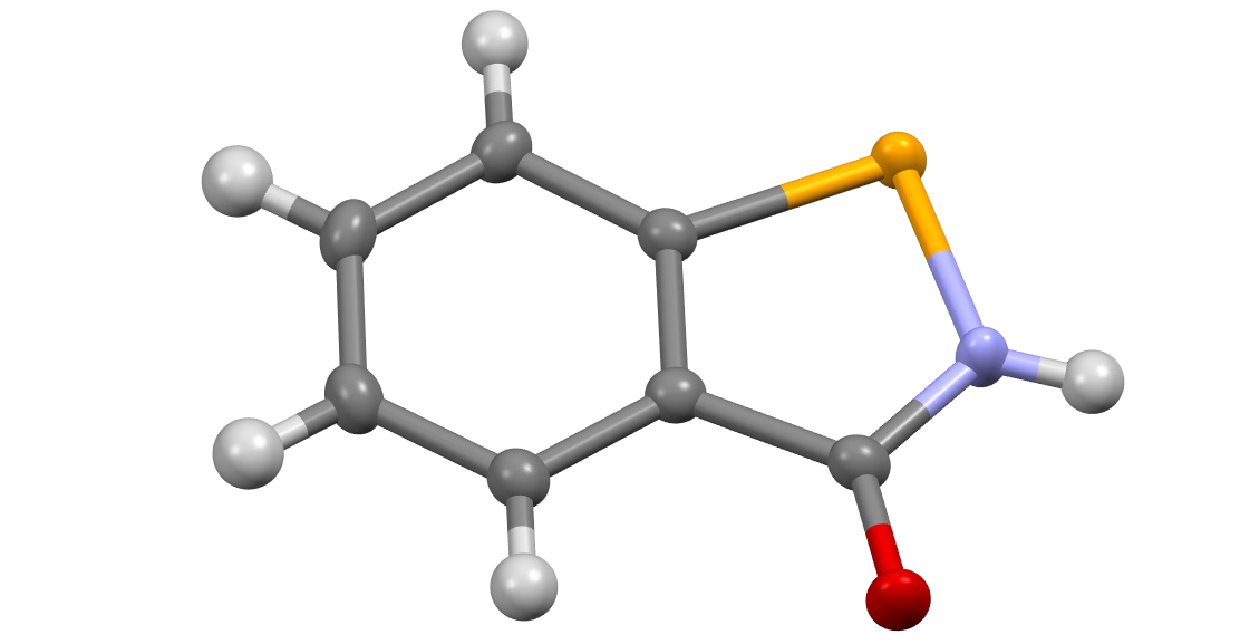
\includegraphics[width=0.8\linewidth]{Figures/ebs-h-xtal.pdf}
    \caption{X-ray crystal structure of \refcmpd{ebs.h}.}
\end{figure}

\ce{C7 H5 N O Se}, $M=198.08$, $T=100(1)$~K, $\lambda=1.54184$~\AA, monoclinic, space group $\text{P}2_1/\text{n}$ (no. 14), $a = 8.7887(2)$~\AA, $b = 6.71260(10)$~\AA, $c = 12.2004(2)$~\AA, $\alpha = 90$\degree, $\beta = 107.285(2)$\degree, $\gamma = 90$\degree, $V = 687.26(2)$~\AA$^{3}$, $Z = 4$. $D_{c}= 1.914$~mg~M$^{-3}$, $\mu$(Cu K\a) = 6.757~mm$^{-1}$, F(000) = 384, crystal size $0.085 \times 0.172 \times 0.214$~mm. 4069 reflections measured, $2\theta_{\mathrm{max}}=152.99$\degree, 1409 independent reflections, R\textsubscript{int} = 0.0261, the final R was 0.0259 ($I > 2\theta(I)$, 1360 reflections) and \emph{w}R(F\textsuperscript{2}) was 0.0732 (all data), GOF 1.122. 

\subsubsection{Preparation of \refcmpd{ebs.thio}}
%TF-7-12
To a sealed tube containing 4~\AA\ molecular sieves (740.7~mg) was added copper (I) iodide (34.3~mg, 0.180~mmol), DMEDA (27.6~mg, 31.3~mmol), potassium carbonate (305.3~mg, 2.209~mmol), benzisothiazolinone \cmpd{ebs.thio}, bromobenzene (190.6~mg, 1.213~mmol), and dioxane (3~mL).
The tube was capped and heated to 120\degree{}C for 18~h, then cooled and the mixture tipped into water (30~mL). The resulting blue suspension was centrifuged, and the blue supernatant discarded. The residue was dissolved in 1:1 DCM/methanol, and decanted off from the sieves.
The solvent was evaporated to afford a greenish solid, which was chromatographed to give the product as colourless needles (105.0~mg, 45\%).\autocite{Dahl2011}

\ce{^{1}H}-NMR (400~MHz, \ce{\emph{d}6}-DMSO) $\delta$ ppm 8.05 (1H, d, \emph{J} = 8.2~Hz), 7.94 (1H, d, \emph{J} = 7.75~Hz), 7.75 (1H, t, \emph{J} = 7.69~Hz), 7.69 (2H, d, \emph{J} = 8.13~Hz), 7.56--7.46 (3H, m), 7.36 (1H, t, \emph{J} = 7.39~Hz).

MS (ESI +ve) m/z 228.0476 (\ce{MH+}) \ce{C13H10NOS+} requires 228.0478 ($\Delta=0.88$~ppm).

\subsubsection{Preparation of \refcmpd{bromodiamine}}
The nitrobenzene (4.9982~g, 23.031~mmol) was dissolved in ethanol (35~mL), and to this was added tin (II) chloride dihydrate (26.022~g, 115.25~mmol, 5~eq).
The mixture was refluxed for 8~h, then cooled, concentrated, and diluted with water to a volume of 300~mL.
The thick white suspension was basified to pH 12, cooled again, and extracted with diethyl ether ($2\times200$~mL).
The combined organic layers were washed with brine (150~mL), dried (\ce{MgSO4}), and evaporated to give a brownish oil, which was triturated with petroleum ether to give a light yellow solid which was used without further purification (3.9759~g, 92\%).\autocite{Urban2011}

\ce{^{1}H}-NMR (400~MHz, \ce{\emph{d}6}-DMSO) $\delta$ ppm 6.6 (1H, d, \emph{J} = 2.17~Hz), 6.47--6.42 (1H, dd, \emph{J} = 2.17, 8.2~Hz), 6.39 (1H, d, \emph{J} = 8.2~Hz), 4.61 (4H, br.\ s.).

\subsubsection{Preparation of \refcmpd{rhs-bromo-2py}}
A 0.1~M solution of sodium methoxide was prepared by dissolving sodium metal (137~mg) in anhydrous methanol (50~mL).
Of this, 6.8~mL was added to 2-pyridine carbonitrile (714.0~mg, 6.858~mmol) and the mixture heated to 80\degree{}C under an argon atmosphere for 1~h to afford the carboximidate \cmpd{2py-carboximidate}.
To this was then added a solution of the diamine \cmpd{bromodiamine} (1.0226~g, 5.467~mmol) in a further 20~mL anhydrous methanol, followed by glacial acetic acid (650~$\mu$L, 11.5~mmol), and the mixture gently refluxed for 18~h.
Upon cooling, the mixture was concentrated to give a yellow oil which was triturated with 1~M aqueous ammonia to give a friable pale yellow solid, which was washed with water to give the product (1.3595~g, 91\%).\autocite{Conn2011}

\ce{^{1}H}-NMR (400~MHz, \ce{\emph{d}6}-DMSO + \textit{d}-TFA vapour) $\delta$ ppm 8.72 (1H, d, \emph{J} = 4.21~Hz), 8.31 (1H, d, \emph{J} = 7.85~Hz), 8.01 (1H, t, \emph{J} = 7.7~Hz), 7.79 (1H, s), 7.63--7.49 (2H, m), 7.37 (1H, d, \emph{J} = 8.53~Hz).

MS (ESI +ve) m/z 273.9975 (\ce{MH+}) \ce{C12H9BrN3+} requires 273.9974 ($\Delta=0.36$~ppm).

\subsubsection{Preparation of \refcmpd{rhs-bromo-2py.pmb}}
The benzimidazole \cmpd{rhs-bromo-2py} (1034.1~mg, 3.797~mmol) and sodium hydride (60\% in oil, 298.2~mg, 7.450~mmol, 2.5~eq) were dissolved in anhydrous DMF (6~mL) at 0\degree{}C, and to this was added \textit{p}-methoxybenzyl chloride (600~$\mu$L, 4.42~mmol, 1.2~eq).
The mixture was warmed to room temperature and stirred for 18~h, then diluted with water (50~mL) and extracted with DCM ($2\times80$~mL).
The combined organic phases were washed with brine, dried (\ce{MgSO4}) and evaporated to give a yellow oil, which was chromatographed to afford two major fractions which when combined gave a 82\% overall yield:
\begin{enumerate}
    \item 633~mg.
    
    \ce{^{1}H}-NMR (599~MHz, \ce{CDCl3}) $\delta$ ppm 8.68 (1H, d, \textit{J} = 4.63~Hz), 8.4 (1H, d, \textit{J} = 7.96~Hz), 7.99 (1H, d, \textit{J} = 1.41~Hz), 7.86 (1H, dt, \textit{J}\textsubscript{1} = 1.39~Hz, \textit{J}\textsubscript{2} = 7.76~Hz), 7.4--7.33 (2H, m), 7.23 (1H, d, \textit{J} = 8.61~Hz), 7.11 (2H, d, \textit{J} = 8.55~Hz), 6.78 (2H, d, \textit{J} = 8.64~Hz), 6.1 (2H, s), 3.75 (3H, s).

    \ce{^{13}C}-NMR (150~MHz, \ce{CDCl3}) $\delta$ ppm 159.0, 150.86, 150.18, 148.73, 144.04, 136.99, 135.7, 129.07, 128.16, 126.51, 124.92, 124.16, 122.89, 115.73, 114.04, 112.1, 55.23, 48.53.

    \item 591~mg.
    
    \ce{^{1}H}-NMR (599~MHz, \ce{CDCl3}) $\delta$ ppm 8.66 (1H, dq, \textit{J}\textsubscript{1} = 0.90~Hz, \textit{J}\textsubscript{2} = 4.80~Hz), 8.41 (1H, dt, \textit{J}\textsubscript{1} = 1.10~Hz, \textit{J}\textsubscript{2} = 7.91~Hz), 7.85 (1H, td, \textit{J}\textsubscript{1} = 1.82~Hz, \textit{J}\textsubscript{2} = 7.78~Hz), 7.71 (1H, dd, \textit{J}\textsubscript{1} = 0.47~Hz, \textit{J}\textsubscript{2} = 8.57~Hz), 7.53 (1H, d, \textit{J} = 1.81~Hz), 7.42 (1H, dd, \textit{J}\textsubscript{1} = 1.83~Hz, \textit{J}\textsubscript{2} = 8.57~Hz), 7.35 (1H, ddd, \textit{J}\textsubscript{1} = 1.15~Hz, \textit{J}\textsubscript{2} = 4.81~Hz, \textit{J}\textsubscript{3} = 7.57~Hz), 7.13 (2H, d, \textit{J} = 8.88~Hz), 6.8 (2H, d, \textit{J} = 8.82~Hz), 6.07 (2H, s), 3.76 (3H, s).

    \ce{^{13}C}-NMR (150~MHz, \ce{CDCl3}) $\delta$ ppm 159.01, 150.57, 150.2, 148.72, 141.71, 137.85, 136.96, 128.98, 128.15, 126.19, 124.8, 124.11, 121.37, 116.77, 114.09, 113.8, 55.23, 48.52.
    
\end{enumerate}

MS (ESI +ve) m/z 394.0555 (\ce{MH+}) \ce{C20H17BrN3O+} requires 394.0550 ($\Delta=1.27$~ppm).

\begin{figure}
    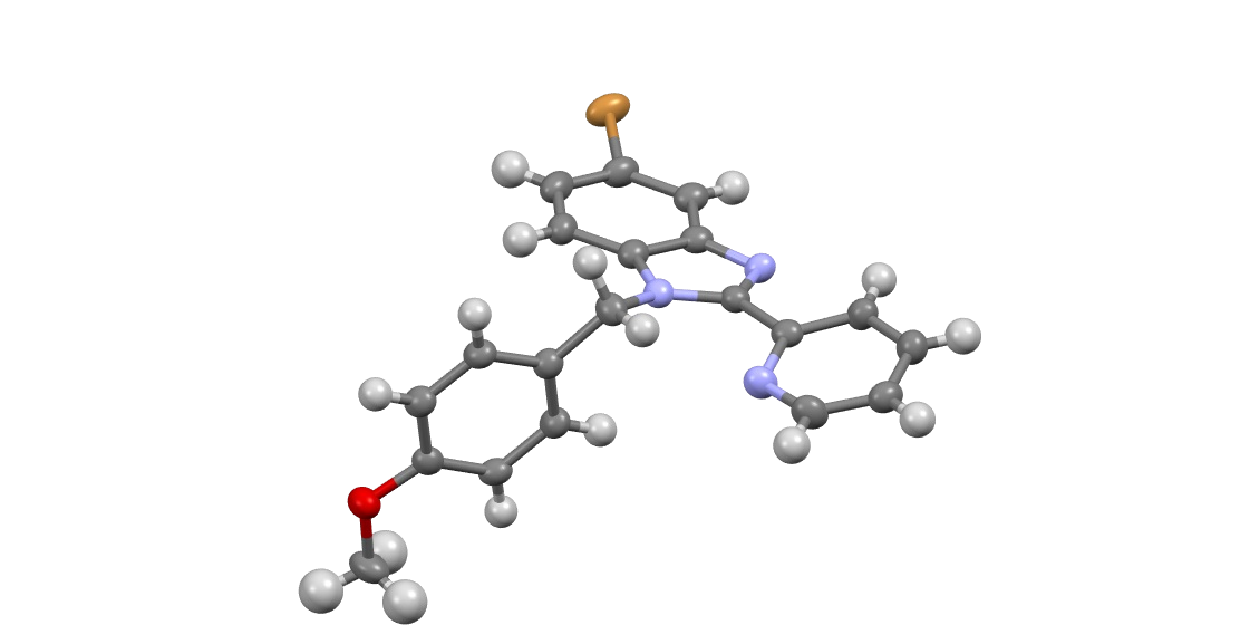
\includegraphics[width=0.8\linewidth]{Figures/rhs-bromo-2py-pmb-xtal.pdf}
    \caption{X-ray crystal structure of \refcmpd{rhs-bromo-2py.pmb}.}
\end{figure}

\ce{C20 H16 Br N3 O}, $M=394.27$, $T=100.00(10)$~K, $\lambda=1.54184$~\AA, monoclinic, space group $\text{P}2_1/\text{n}$ (no. 14), $a = 13.2476(4)$~\AA, $b = 9.0084(2)$~\AA, $c = 14.1474(5)$~\AA, $\alpha = 90$\degree, $\beta = 91.033(3)$\degree, $\gamma = 90$\degree, $V = 1688.07(9)$~\AA$^{3}$, $Z = 4$. $D_{c}= 1.551$~mg~M$^{-3}$, $\mu$(Cu K\a) = 3.420~mm$^{-1}$, F(000) = 800, crystal size $0.04 \times 0.072 \times 0.118$~mm. 10353 reflections measured, $2\theta_{\mathrm{max}}=153.936$\degree, 3452 independent reflections, R\textsubscript{int} = 0.0453, the final R was 0.0469 ($I > 2\theta(I)$, 2896 reflections) and \emph{w}R(F\textsuperscript{2}) was 0.1237 (all data), GOF 1.032. 

\subsubsection{Preparation of \refcmpd{rhs-bromo-ph}}
Sodium metabisulfite (9.670~g, 50.85~mmol) was dissolved in 50~mL water and added to 200~mL ethanol, then benzaldehyde (5.444~g, 51.30~mmol) was added.
This was stirred at room temperature for 1~h, then a solution of the diamine \cmpd{bromodiamine} (4.0437~g, 21.6~mmol) in ethanol (40~mL) was added, and the mixture refluxed under nitrogen for 24~h, then cooled and left to stand for 60~h.
The solvent was removed by rotary evaporator, and the residue triturated with 1~M aqueous ammonia (50~mL). 
The resulting precipitate was filtered off, washed with water ($2\times25$~mL), cold diethyl ether (5~mL), and dried affording the benzimidazole \cmpd{rhs-bromo-ph} (5.1646~g, 79\%).\autocite{Kim2011}

\ce{^{1}H}-NMR (499~MHz, \ce{\emph{d}6}-DMSO + \textit{d}-TFA) $\delta$ ppm 8.18 (2H, d, \emph{J} = 6.89~Hz), 7.83 (1H, s), 7.64--7.52 (4H, m), 7.41 (1H, dd, \emph{J}\textsubscript{1} = 1.51~Hz, \emph{J}\textsubscript{2} = 8.52~Hz).

\subsubsection{Preparation of \refcmpd{ebs-rhs-ph.thio-pmb}}
Benzisothiazolinone \cmpd{ebs.h-thio} (173.1~mg, 1.142~mmol), aryl bromide \cmpd{rhs-bromo-ph.pmb} (401.9~mg, 1.022~mmol), 4~\AA\ molecular sieves (607.1~mg), DMEDA (32.7~mg, 0.371~mmol), potassium carbonate (283.8~mg, 2.053~mmol), and dioxane (3~mL) were combined in a sealed tube under a nitrogen atmosphere, and heated at 120\degree{}C for 24~h.
The mixture was then cooled to room temperature and tipped into water (40~mL).
The suspension was centrifuged, and the supernatant discarded, then the residue redissolved in methanol ($2\times40$~mL).
This was filtered, and the filtrate evaporated to give a light brown oil, which was applied to a SNAP 25~g silica cartridge and eluted with an ethyl acetate/petroleum ether gradient to give two fractions:
\begin{enumerate}
    \item 160.9~mg, aryl bromide \cmpd{rhs-bromo-ph.pmb},
    \item 231.2~mg, 48\%, benzisothiazolinone-benzimidazole \cmpd{ebs-rhs-ph.thio-pmb}.
\end{enumerate}

\cmpd{ebs-rhs-ph.thio-pmb} crystallised in two distinct polymorphs:
\begin{enumerate}
    \item P$\bar{1}$, m.p. 101.0--104.2\degree{}C
    \item P$2_1$/n, m.p. 134.1--138.4\degree{}C
\end{enumerate}

\ce{^{1}H}-NMR (600~MHz, \ce{\emph{d}6}-DMSO) $\delta$ ppm 8.03 (1H, d, \emph{J} = 8.08~Hz), 7.92 (1H, d, \emph{J} = 7.67~Hz), 7.86--7.79 (2H, m), 7.73 (3H, d, \emph{J} = 4.68~Hz), 7.55 (3H, d, \emph{J} = 3.42~Hz), 7.51--7.44 (2H, m), 6.93 (2H, d, \emph{J} = 8.38~Hz), 6.82 (2H, d, \emph{J} = 8.46~Hz), 5.52 (2H, s), 3.66 (3H, s).

\ce{^{13}C}-NMR (150~MHz, \ce{CDCl3}) $\delta$ ppm 163.89, 159.7, 155.30, 142.13, 140.79, 136.40, 132.92, 132.31, 130.56, 130.37, 129.57, 129.34, 128.90, 127.97, 122.36, 120.63, 120.33, 114.69, 109.04, 55.50, 47.55.

MS (ESI +ve) m/z 464.1431 (\ce{MH+}) \ce{C28H22N3O2S+} requires 464.1427 ($\Delta=0.86$~ppm).

CRYSTAL DATA HERE???

\subsubsection[Preparation of \refcmpd{rhs-nitro-amide}]{Preparation of N-(2-amino-5-nitrophenyl)benzamide \refcmpd{rhs-nitro-amide}}
4-Nitro-1,2-benzenediamine (3.0797~g, 20.110~mmol) and TEA (3~mL, distilled from \ce{CaH2}) were dissolved in anhydrous THF (150~mL).
Benzoyl chloride (1.5~mL, 1.8~g, 13~mmol) was then added at $-10$\degree{}C and the mixture slowly warmed to room temperature while stirring for 18~h.
The mixture was then tipped into water (400~mL), and extracted with ethyl acetate ($3\times100$~mL).
The combined organic layers were washed with water ($2\times200$~mL), brine (200~mL), then dried (\ce{MgSO4}) and evaporated to give a reddish solid.
This was recrystallised from ethyl acetate to give the amide \cmpd{rhs-nitro-amide} as yellow crystals (2.5027~g, 75\%).\autocite{Patrick2017}

\ce{^1H}-NMR (400~MHz, DMSO-\emph{d6}) $\delta$ 9.66 (s, 1H), 8.04 (s, 1H), 7.92 (d, J = 7.4 Hz, 2H), 7.83 (d, J = 9.2 Hz, 1H), 7.50 (d, J = 6.8 Hz, 1H), 7.44 (t, J = 7.3 Hz, 2H), 6.71 (d, J = 9.0 Hz, 1H), 6.52 (s, 2H).

\subsubsection[Preparation of \refcmpd{rhs-nitro}]{Preparation of 6-nitro-2-phenyl-1\emph{H}-benzo[\emph{d}]imidazole \refcmpd{rhs-nitro}}
%TF-7-94-CP
Amide \cmpd{rhs-nitro-amide} (1.2283~g, 4.7749~mmol) was refluxed in a solution of \ce{BF3\cdot OEt2} (0.75~mL) and dioxane (75~mL) for 1.5~h.
The mixture was then cooled to room temperature, stirred for 18~h, then heated to reflux again for 2~h.
The yellow solution was diluted with water (300~mL) and extracted with ethyl acetate ($3\times75$~mL),
The combined organic layers were washed with water and brine (100~mL each), then dried (\ce{Na2SO4}), and evaporated to give a brown oil.
Trituration with petroleum spirit/dichloromethane afforded \cmpd{rhs-nitro} as a light brown friable solid (1.0606~g, 93\%).\autocite{Patrick2017}

\ce{^1H}-NMR (400~MHz, DMSO-\emph{d6} + \textit{d}-TFA) $\delta$ 8.47 (s, 1H), 8.21 (q, J = 3.2 Hz, 2H), 8.13 (q, J = 3.7 Hz, 1H), 7.76 (d, J = 8.9 Hz, 1H), 7.54--7.62 (m, 3H).

MS (ESI +ve) m/z 240.0768 (\ce{MH+}) \ce{C13H10N3O2+} requires 240.0768 ($\Delta=0$~ppm).

\begin{figure}[ht]
    \centering
    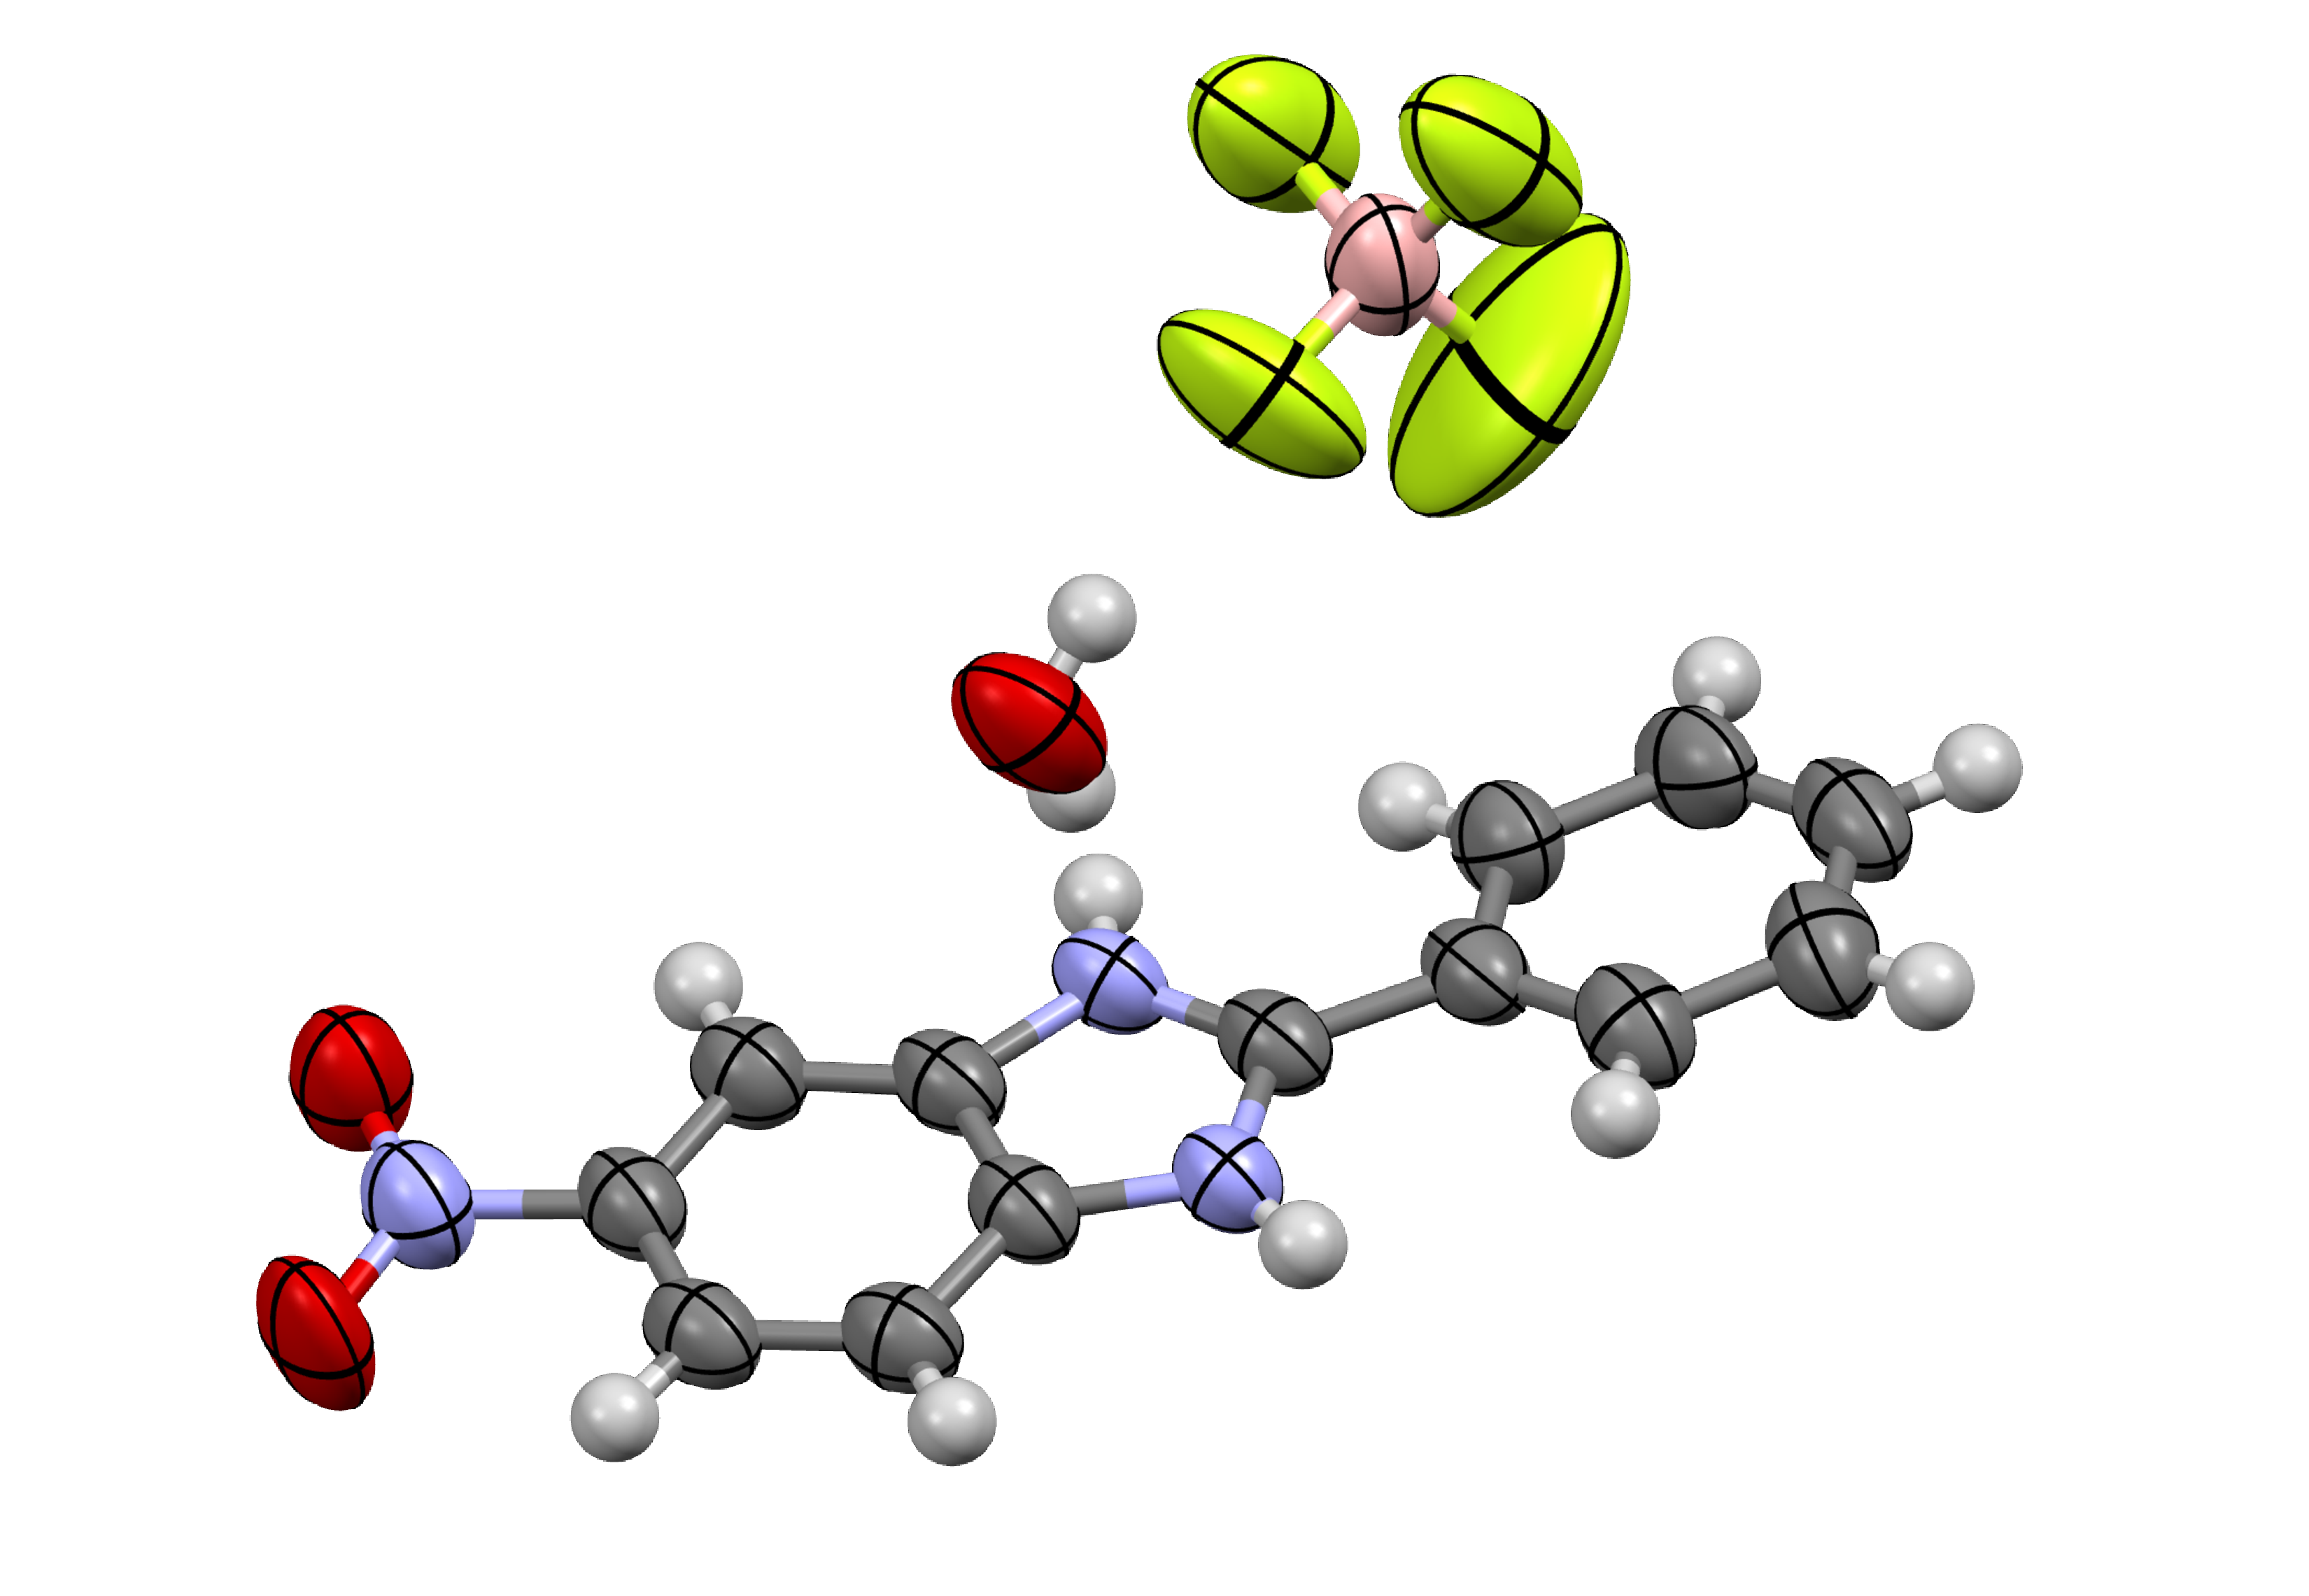
\includegraphics[width=0.8\linewidth]{Figures/rhs-nitro-xray.pdf}
    \caption{X-ray crystal structure of \refcmpd{rhs-nitro} as the tetrafluoroborate salt.}\label{fig:rhs-nitro-xray}
\end{figure}

\ce{C13 H12 B F4 N3 O3}, $M=345.07$, $T=100.3(9)$~K, $\lambda=1.54184$~\AA, monoclinic, space group $\text{P}2_1/\text{c}$ (no. 14), $a = 7.6592(2)$~\AA, $b = 16.1459(4)$~\AA, $c = 11.7238(2)$~\AA, $\alpha = 90$\degree, $\beta = 96.208(2)$\degree, $\gamma = 90$\degree, $V = 1441.32(6)$~\AA$^{3}$, $Z = 4$. $D_{c}= 1.590$~mg~M$^{-3}$, $\mu$(Cu K\a) = 1.288~mm$^{-1}$, F(000) = 704, crystal size $0.057 \times 0.084 \times 0.189$~mm. 9706 reflections measured, $2\theta_{\mathrm{max}}=154.124$\degree, 2966 independent reflections, R\textsubscript{int} = 0.0266, the final R was 0.0748 ($I > 2\theta(I)$, 2549 reflections) and \emph{w}R(F\textsuperscript{2}) was 0.2084 (all data), GOF 1.065. 

\subsubsection[Preparation of \refcmpd{rhs-amine}]{Preparation of 2-phenyl-1\emph{H}-benzo[\emph{d}]imidazol-6-amine \refcmpd{rhs-amine}}
%TF-7-117-CP
A solution of the nitrobenzene \cmpd{rhs-nitro} (893.6~mg, 3.735~mmol) and tin (II) chloride dihydrate (4.410~g, 19.54~mmol) in concentrated hydrochloric acid (20~mL) was refluxed for 2~h.
The solution was then cooled, and basified to pH 10 using 5~M aqueous sodium hydroxide.
This was then extracted with ethyl acetate ($2\times30$~mL), washing with water and brine (30~mL each).
The combined organic layers were dried (\ce{Na2SO4}) then evaporated to give \cmpd{rhs-amine} as a brownish solid (677.2~mg, 87\%).\autocite{Patrick2017}

\ce{^{1}H}-NMR (400~MHz, \ce{\textit{d}6}-DMSO) $\delta$ ppm 8.19--7.98 (2H, m), 7.62 (3H, d, \textit{J} = 6.54~Hz), 7.53 (1H, d, \textit{J} = 8.66~Hz), 7.07 (1H, s), 6.93 (1H, d, \textit{J} = 8.59~Hz).

MS (ESI +ve) m/z 210.1026 (\ce{MH+}) \ce{C13H12N3+} requires 210.1026 ($\Delta=0$~ppm).

\begin{figure}[ht]
    \centering
    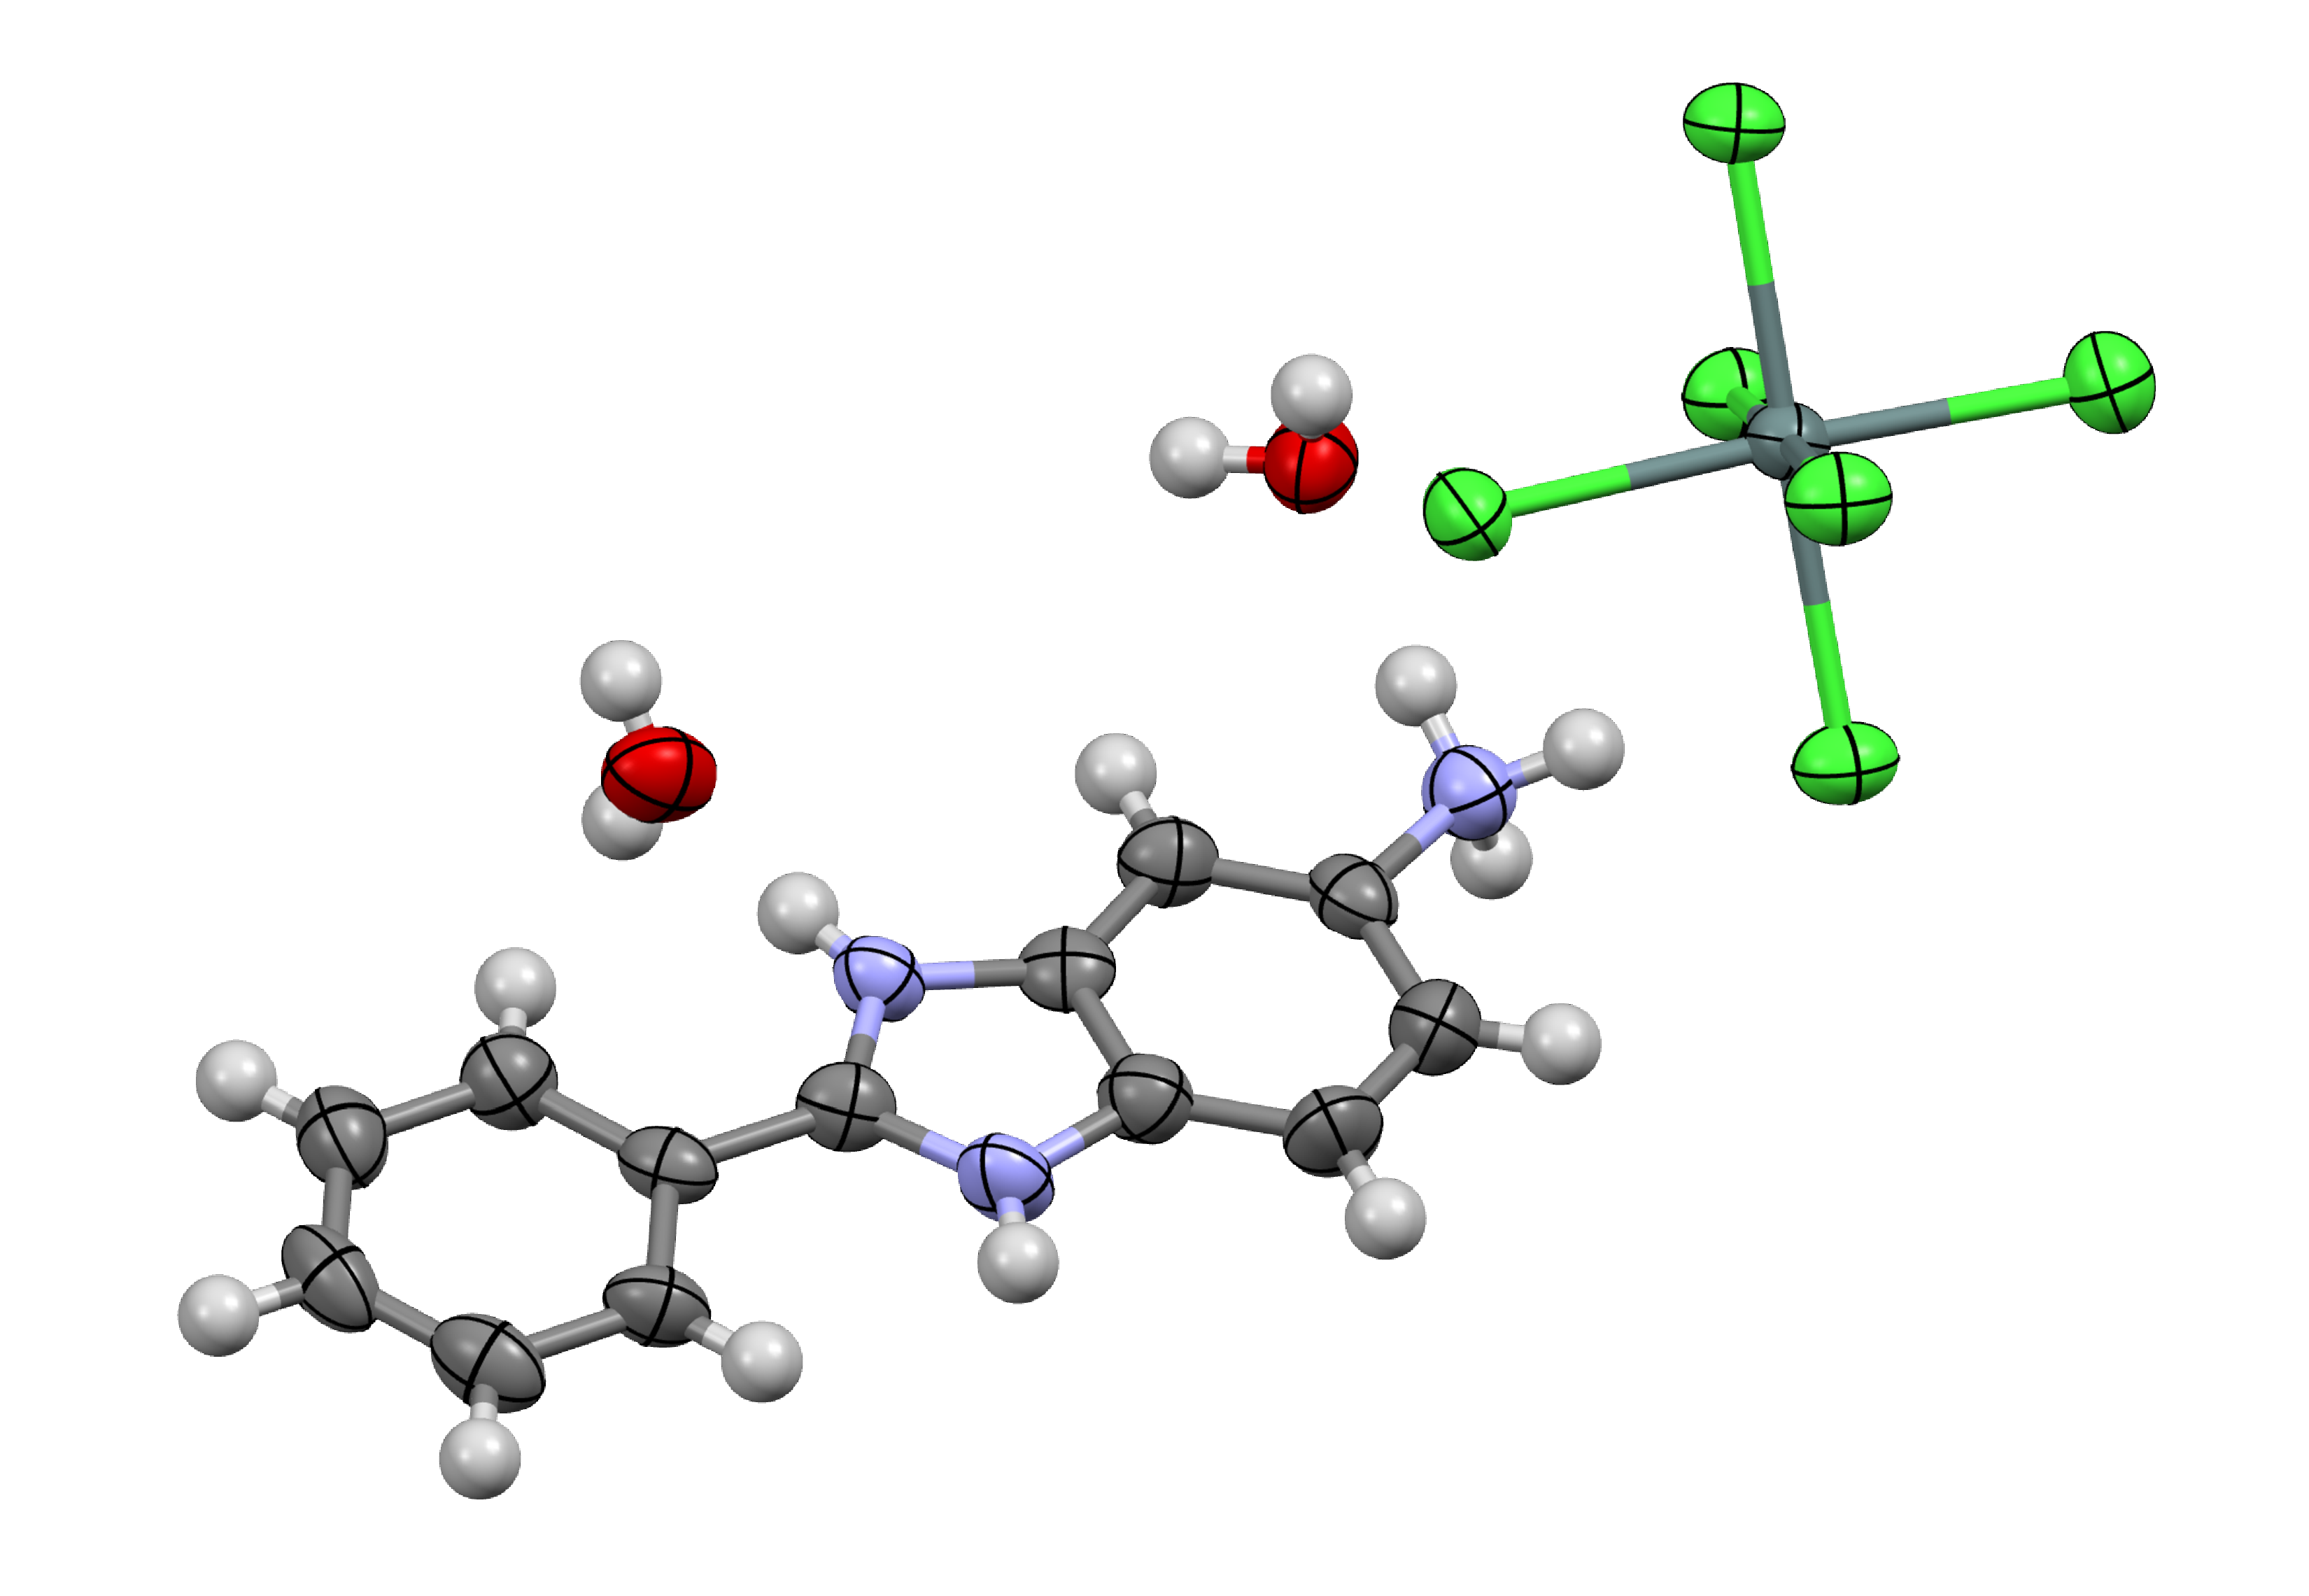
\includegraphics[width=0.8\linewidth]{Figures/rhs-amine-xray.pdf}
    \caption{X-ray crystal structure of \refcmpd{rhs-amine} as the hexachlorostannate salt.}\label{fig:rhs-amine-xray}
\end{figure}

\ce{C13 H17 Cl6 N3 O2 Sn}, $M=578.68$, $T=99.98(10)$~K, $\lambda=1.54184$~\AA, monoclinic, space group $\text{P}2_1/\text{c}$ (no. 14), $a = 6.93400(10)$~\AA, $b = 24.1777(4)$~\AA, $c = 12.2079(3)$~\AA, $\alpha = 90$\degree, $\beta = 97.186(2)$\degree, $\gamma = 90$\degree, $V = 2030.56(7)$~\AA$^{3}$, $Z = 4$. $D_{c}= 1.893$~mg~M$^{-3}$, $\mu$(Cu K\a) = 17.403~mm$^{-1}$, F(000) = 1136, crystal size $0.026 \times 0.032 \times 0.267$~mm. 7450 reflections measured, $2\theta_{\mathrm{max}}=154.058$\degree, 7450 independent reflections, R\textsubscript{int} = ?, the final R was 0.0515 ($I > 2\theta(I)$, 6356 reflections) and \emph{w}R(F\textsuperscript{2}) was 0.1626 (all data), GOF 1.095. 

\subsubsection[Preparation of \refcmpd{ebs-rhs-ph}]{Preparation of 2-(2-phenyl-1\emph{H}-benzo[\emph{d}]imidazol-6-yl)benzo[\emph{d}][1,2]\-selenazol-3(2\emph{H})-one \refcmpd{ebs-rhs-ph}}
%TF-7-188-C1F1
Diselenide \cmpd{diselenide} (440.1~mg, 1.100~mmol) was refluxed in thionyl chloride with 2 drops DMF for 2~h.
The excess reagent was removed by vacuum distillation, and the residue was dissolved in anhydrous acetonitrile (10~mL).
This was added drop-wise to a solution of the aniline \cmpd{rhs-amine} (440.4~mg, 2.105~mmol) and TEA (2~mL) in a further 10~mL anhydrous acetonitrile.
The mixture was stirred at room temperature for 18~h, then briefly brought to reflux.
It was then cooled, diluted with water (30~mL) and extracted into ethyl acetate ($3\times50$~mL).
The combined organic layers were washed with water and brine (50~mL each), then dried (\ce{MgSO4}), then evaporated onto celite.
This was chromatographed on a SNAP 25~g silica cartridge using an ethyl acetate/methanol gradient, affording 2 major fractions:
\begin{enumerate}
    \item orange solid, 67.7~mg, 8\%, \cmpd{ebs-rhs-ph}, m.p. 170\degree{}C (dec.)
    \item yellow solid, 166.0~mg, 38\%, starting material \cmpd{rhs-amine}
\end{enumerate}

\ce{^{1}H}-NMR (499~MHz, \ce{\emph{d}6}-DMSO) $\delta$ ppm 8.23--8.17 (2H, m), 8.12 (1H, d, \emph{J} = 8.08~Hz), 8.07 (1H, s), 7.94 (1H, d, \emph{J} = 7.64~Hz), 7.83 (1H, d, \emph{J} = 8.66~Hz), 7.76--7.67 (4H, m), 7.63 (1H, d, \emph{J} = 8.63~Hz), 7.51 (1H, t, \emph{J} = 7.34~Hz).

\ce{^{13}C}-NMR (150~MHz, \ce{CDCl3}) $\delta$ ppm 172.49, 170.82, 165.53, 164.86, 163.38, 138.86, 137.43, 134.88, 133.84, 132.47, 130.4, 129.45, 128.92, 128.37, 127.12, 126.95, 126.72, 126.23, 126.01, 124.13, 123.65, 119.61.

MS (ESI +ve) m/z 392.0298 (\ce{MH+}) \ce{C20H14N3OSe+} requires 392.0297 ($\Delta=0.26$~ppm).

\printbibliography[heading=subbibliography]
\end{refsection}
